\documentclass[a4paper, fontsize = 8pt, landscape]{scrartcl}
\usepackage{../../../misc_files/LateX/layout_and_colours}
\makeatletter
\def\input@path{{content/lecture_summary/}{content/examples/}}
\makeatother
\graphicspath{{content/images/}{content/lecture_summary/images/}{content/examples/images/}}

\title{Machine Learning and Data Mining}
\author{Jil Zerndt}
\date{FS 2025}

\createtitlepagestyle
\createmainpagestyle
\begin{document}
\begin{multicols}{2}
	\thispagestyle{TitlePageStyle}
	\maketitle
	\sffamily
	


\section{Overview of IT Security}

\mult{2}

\begin{definition}{Key IT Security Goals}
Information security is based on three fundamental principles, commonly known as the CIA triad:
\begin{itemize}
    \item \textbf{Confidentiality} - Ensuring data is only accessible to authorized users
    \item \textbf{Integrity} - Ensuring data is not modified in an unauthorized way
    \item \textbf{Availability} - Ensuring systems and data are accessible when needed
\end{itemize}
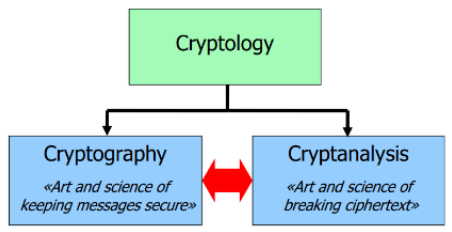
\includegraphics[width=0.6\linewidth]{its_goals.png}
\end{definition}

\begin{concept}{Business IT Risks}
\begin{itemize}
    \item Data loss
    \item System outage
    \item Espionage
    \item Sabotage
    \item Reputation loss
    \item Misuse of computing resources
    \item Violation of regulations
    \item Fraud
    \item Brand misuse
    \item Ransom demands
\end{itemize}
These risks can have significant financial, operational, and reputational impacts.
\end{concept}

\multend

\raggedcolumns

\subsubsection{Security Frameworks and Controls}

\mult{2}

\begin{concept}{Security Control Frameworks}
Security frameworks provide structured approaches to implementing security controls:
\begin{itemize}
    \item \textbf{CIS Controls} - Prioritized set of actions to protect organizations
    \item Controls are typically organized in implementation groups based on difficulty and impact
    \item Focus on preventing the most common attack vectors first
\end{itemize}
\end{concept}

\begin{definition}{Types of Security Measures}
Security measures can be categorized based on their focus:
\begin{itemize}
    \item \textbf{Preventive} - Block threats before they occur (firewalls, access controls)
    \item \textbf{Detective} - Identify when a breach has occurred (IDS, audit logs)
    \item \textbf{Corrective} - Mitigate damage after an incident (backups, incident response)
\end{itemize}
\end{definition}

\multend

\subsubsection{Disaster Recovery}



\begin{concept}{Business Continuity Management}
Disaster recovery and business continuity planning are essential for maintaining availability:
\begin{itemize}
    \item \textbf{Recovery Plan} - Detailed procedures for recovering from incidents
    \item \textbf{Recovery Tests} - Regular testing of recovery procedures
    \item \textbf{Redundancy} - Duplicate systems, power supplies, and network connections
    \item \textbf{Offline backups} - Protection against ransomware and other threats
\end{itemize}
\end{concept}

\begin{KR}{Disaster Recovery Planning}
\paragraph{Initial Assessment}
\begin{itemize}
    \item Identify critical systems and data
    \item Determine acceptable recovery time objectives (RTO)
    \item Determine acceptable recovery point objectives (RPO)
\end{itemize}

\paragraph{Plan Development}
\begin{itemize}
    \item Document recovery procedures
    \item Assign roles and responsibilities
    \item Include contact details for all relevant parties
    \item Develop technical instructions for restoration
\end{itemize}

\paragraph{Testing}
\begin{itemize}
    \item Conduct regular theoretical dry runs
    \item Perform practical tests (e.g., server shutdown, data restoration)
    \item Update procedures based on test results
\end{itemize}

\paragraph{Regular Review}
\begin{itemize}
    \item Review and update plans regularly
    \item Consider changes in infrastructure, personnel, and threats
\end{itemize}
\end{KR}

\begin{example}
A medium-sized company implements a disaster recovery plan for their customer database. They define an RTO of 4 hours and an RPO of 15 minutes, meaning they need to restore service within 4 hours with no more than 15 minutes of data loss. To achieve this, they implement a combination of hourly differential backups with continuous transaction log shipping to a standby site. Regular recovery tests are scheduled quarterly to ensure the plan remains effective.
\end{example}

\mult{2}


\begin{concept}{Problems - Overview}\\ and their impact on data availability
\paragraph{Physisch}
\textbf{unabsichtlich}
\begin{itemize}
    \item Naturkatastrophen
    \item Feuer
    \item Ausfall
    \item Kaffee auf Server
\end{itemize}

\textbf{absichtlich/bösartig}
\begin{itemize}
    \item Feuer
    \item Vandalismus
    \item Garantie läuft aus -> absichtlich langsamer
    \item Social Engineering
\end{itemize}

\paragraph{Virtuell}
\textbf{unabsichtlich}
\begin{itemize}
    \item Bitflip
    \item Config Fehler
    \item Bugs im SW
    \item Phishing klicken
\end{itemize}

\textbf{absichtlich/bösartig}
\begin{itemize}
    \item DDoS
    \item Malware
    \item Ransomware
    \item Phishing senden
    \item Trojaner
\end{itemize}
\end{concept}

\begin{theorem}{Countermeasures - Overview}

\textbf{Disaster Recovery}
    \begin{itemize}
        \item Offline backup solutions
        \item Restoring from images
    \end{itemize}

\textbf{Access Control}
    \begin{itemize}
        \item Restricted Access Rights
        \item Multi-Factor Authentication
        \item Firewalls
        \item Traffic Management Solutions
    \end{itemize}

\textbf{Physical Protection}
    \begin{itemize}
        \item Physical Access Control (locks, fences, etc.)
        \item Fire Protection (extinguishers, alarms, etc.)
        \item Monitoring (CCTV, Guards etc.)
    \end{itemize}

\textbf{Training Processes}
    \begin{itemize}
        \item Employee Training
        \item Four eyes principle
        \item Automation of routine processes
        \item Monitoring
        \item Preventive maintenance
    \end{itemize}

\textbf{Redundancy}
    \begin{itemize}
        \item Uninterruptable Power Supplies
        \item High Availability setups
        \item Load Balancing
        \item Redundant data center
        \item Redundant network connections
    \end{itemize}
\end{theorem}

\multend

\mult{2}

\begin{formula}{Recovery Plan and Test}

    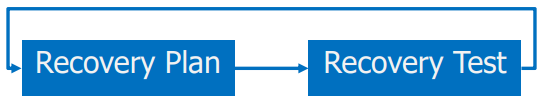
\includegraphics[width=0.7\linewidth]{recovery_plan_test.png}

    \textbf{Recovery Plan} - description of what to do if something goes wrong
    \begin{itemize}
        \item Roles and responsibilities
        \item Processes
        \item Contact details
        \item Technical instructions
    \end{itemize}

    \textbf{Recovery Test} - testing the recovery plan
    \begin{itemize}
        \item Theoretical dry run
        \item Practical tests
        \begin{itemize}
            \item turn off a server or DC
            \item restore data from backup
        \end{itemize}
    \end{itemize}
\end{formula}

\begin{concept}{Goals of IT Security}

Most measures in Information Security have one of the three following high-level goals:
\begin{itemize}
    \item Ensure data is confidential
    \item Ensure data is not corrupted
    \item Ensure data and systems are available
\end{itemize}

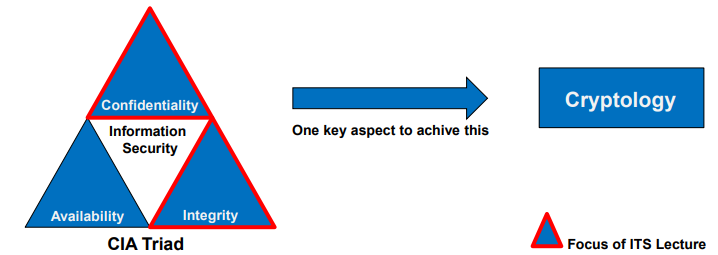
\includegraphics[width=\linewidth]{goals_of_IT_security.png}
\end{concept}

\multend

\raggedcolumns





	\raggedcolumns
	\pagebreak
	\section{Data Preprocessing}

\begin{remark}
    Learning Objectives:
    \begin{itemize}
        \item Understand fundamental importance of data preprocessing
        \item Know basic algorithms for data cleaning, (near) duplicate detection and filling missing values
    \end{itemize}
\end{remark}

\subsection{Data-Driven Projects}

\mult{2}

\begin{concept}{Typical Data Driven Project}
    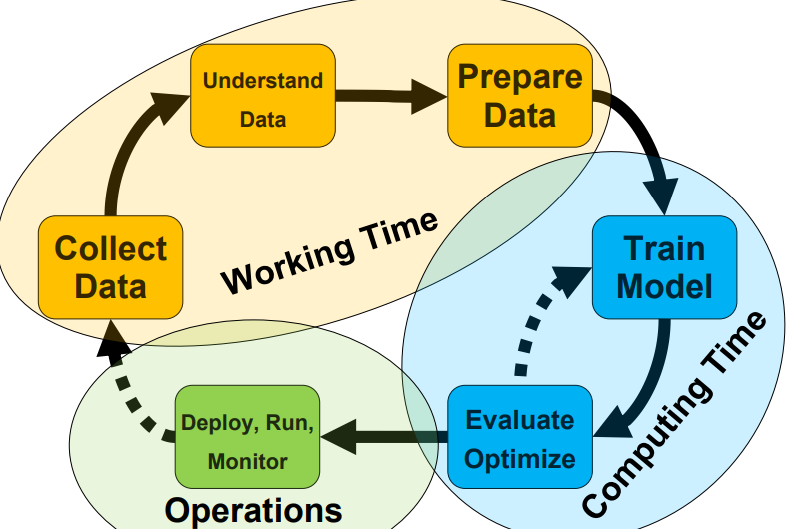
\includegraphics[width=\linewidth]{typical_data_driven_project.png}
\end{concept}

\subsection{Data Types}

\begin{theorem}{Data Types}
    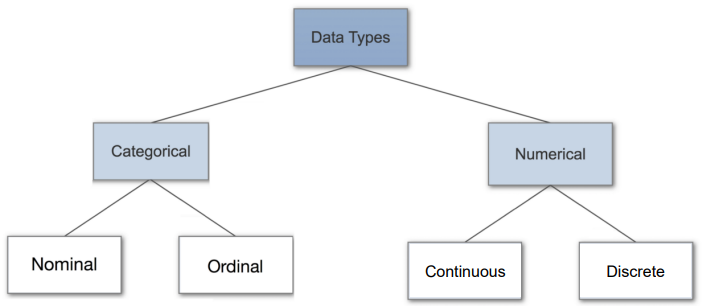
\includegraphics[width=\linewidth]{data_types.png}
\end{theorem}

\begin{concept}{Overview Data Types}
    \textbf{Categorical Data}
    \begin{itemize}
        \item Nominal: no order, Scale ("labels") $\rightarrow$ e.g. hair colour, gender
        \item Ordinal: ordered $\rightarrow$ e.g. military rank, star rating
    \end{itemize}

    \textbf{Numerical Data} (ordered)
    \begin{itemize}
        \item Discrete: countable, ratio $\rightarrow$ e.g. number of persons in a room
        \item Continuous: interval, numeric scale $\rightarrow$ e.g. temperature, weight
    \end{itemize}
\end{concept}

\begin{definition}{Data} has many sources, e.g.: 
    sensor, survey, simulation, social media, textual, financial, multimedia, ERP systems data, etc.
    
    Independent of the data source, each data point has a data type
\end{definition}

\begin{corollary}{Nominal Data}
    \begin{itemize}
        \item Nominal scales are used for \textbf{labelling} variables, without any quantitative value
        \item No numerical significance
        \item Nominal data has no order
        \item Scales could simply be called labels
        \item Examples: gender, hair colour, race, marital status
    \end{itemize}
\end{corollary}

\begin{corollary}{Ordinal Data}
    \begin{itemize}
        \item Represents \textbf{discrete and ordered} units
        \item Nearly the same as nominal data, but \textbf{order matters}
        \item No distance between the different categories
        \item Examples: military rank, star rating, education level
    \end{itemize}
\end{corollary}

\begin{corollary}{Discrete Numeric Data}
    \begin{itemize}
        \item Represents items that can be \textbf{counted}
        \item Values may go from 0, 1, 2, on to infinity (making it countably infinite)
        \item Examples: number of persons in a room, number of "heads" in 60 coin flips, time elapsed in minutes
    \end{itemize}
\end{corollary}

\begin{corollary}{Continuous Numeric Data}
    \begin{itemize}
        \item Also known as \textbf{interval data}
        \item Often measurements
        \item Possible values \textbf{cannot be counted} and can only be described using intervals on the real number line
        \item Examples: temperature, weight, height, time, ...
    \end{itemize}
\end{corollary}

\multend

\subsection{Data Quality}

\begin{formula}{Standard Error Measure}
    $$
    \begin{gathered}
    E=\frac{1}{N} \sum_{i=1}^N\left(1-\text { id }\left(\hat{y}_i, y_i\right)\right), \quad \text { id }(a, b)= \begin{cases}1 & \text { if } a=b \\
    0 & \text { else }\end{cases} \\
    \text { data } a_{\text {size }}=9, \quad \text { correct }=6, \quad \text { wrong }=3 \\
    E=\frac{1}{9} \cdot 3=0.33
    \end{gathered}
    $$
\end{formula}

\subsection{Data Cleaning}

\mult{2}

\begin{definition}{Data Cleaning}
    is the process of improving the data quality by removing or improving incorrect or improperly formatted data.
    \vspace{1mm}\\
    \textbf{(near) duplicate detection} is the process of identifying and removing or merging duplicate data points.
    \begin{itemize}
        \item compare attributes of the tuple
        \item compare content of the attributes
    \end{itemize}
    \vspace{1mm}
    \textbf{Filling missing values} is the process of replacing missing values with substituted values.
    \begin{itemize}
        \item ignore tuple
        \item fill in missing value manually
        \item use global constant such as "unknown" or "-1"
        \item use attribute mean, median, mode
        \item use most probable value
    \end{itemize}
    \vspace{1mm}
    \textbf{Noisy data} is data with errors or outliers.
    \begin{itemize}
        \item Binning: divide the range of attribute values into bins
        \item Regression: smooth data by fitting the data into a function
        \item Clustering: detect and remove outliers
    \end{itemize}
\end{definition}

\subsection{Data Binning}

\begin{formula}{Equal Width Binning}\\
    Divide the range into $N$ intervals of equal size (= width)
    $$width = \frac{max - min}{N}$$
    $$bin_i = [min + i \cdot width, min + (i+1) \cdot width]$$
    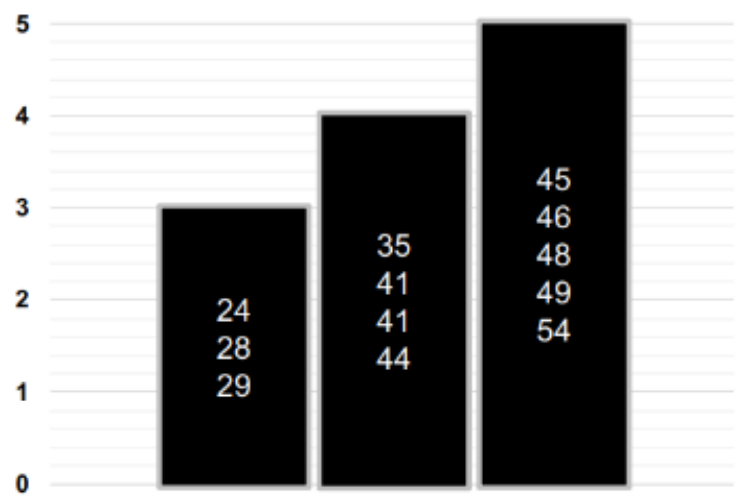
\includegraphics[width=\linewidth]{equal_width_ninning.png}
\end{formula}

\begin{formula}{Equal Depth/Frequency Binning}\\
    Divide the range into $N$ intervals with equal number of data points/records (= depth/frequency)
    $$depth = \frac{N}{n}$$
    $$bin_i = [data_{(i-1) \cdot depth}, data_{i \cdot depth}]$$
    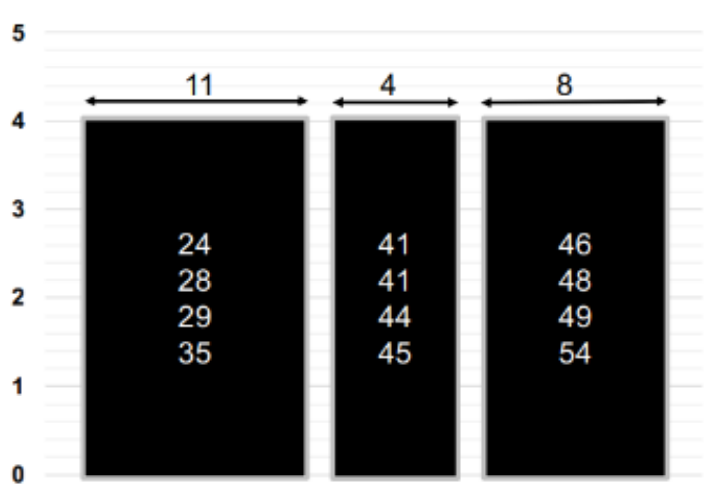
\includegraphics[width=\linewidth]{equal_depth_binning.png}
\end{formula}

\multend

\subsection{Data Normalization}

\begin{definition}{Data Normalization}
    is the process of transforming values of several variables into a similar range.
    $$\text{Min-Max Normalization: } x_{norm} = \frac{x - min(x)}{max(x) - min(x)}$$
    $$\text{Z-Score Normalization: } x_{norm} = \frac{x - \bar{x}}{\sigma}$$
    Change the values of numeric columns to a common scale (e.g., between 0 and 1), without distorting differences in the ranges of values.
    $$\text{Linear Normalization: } f_{lin}(v) = \frac{v - min}{max - min}$$
    $$\text{Square Root Normalization: } f_{sq}(v) = \frac{\sqrt{v} - \sqrt{min}}{\sqrt{max} - \sqrt{min}}$$
    $$\text{Logarithmic Normalization: } f_{ln}(v) = \frac{\ln(v) - \ln(min)}{\ln(max) - \ln(min)}$$

    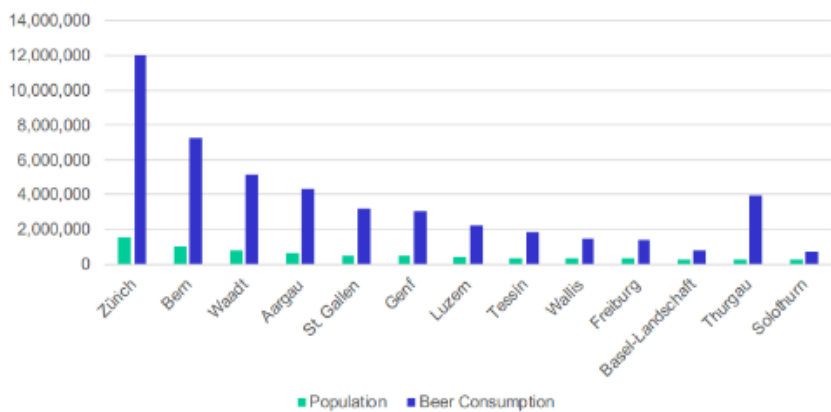
\includegraphics[width=\linewidth]{data_normalization1.png}

    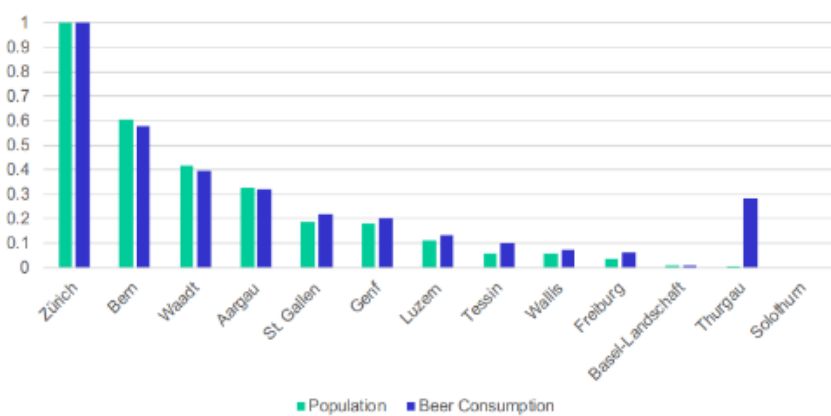
\includegraphics[width=\linewidth]{data_normalization2.png}
\end{definition}

\subsection{Data Sampling}

\begin{definition}{Data Sampling}
    Represent large dataset by smaller subset to speed up automatic calculations.
    \vspace{1mm}\\
    \textbf{Non-Probabilistic}
    \begin{itemize}
        \item Convenience: easiest to obtain
        \item Judgement: based on experts' knowledge and judgement
        \item Snowball: purely based on referrals
        \item Quota: based on attribute values
    \end{itemize}
    \vspace{1mm}
    \textbf{Probabilistic}
    \begin{itemize}
        \item Simple Random: each item has an equal probability of being chosen
        \item Systematic: select some starting point and then select every $k$th element
        \item Stratified: divide the population into subgroups (strata) based on attributes and then draw a sample from each stratum
        \item Cluster: divide the population into clusters and then randomly select some of the clusters
    \end{itemize}
\end{definition}

\subsection{Data Partitioning}

\begin{definition}{Data Partitioning}
    is the process of dividing the dataset into two or more parts.
    \begin{itemize}
        \item Training set: used to train the model
        \item Validation set: used to tune the model
        \item Test set: used to evaluate the model
    \end{itemize}
    \vspace{1mm}
    \textcolor{pink}{\textbf{K-Fold Cross-Validation}}
    \begin{itemize}
        \item Divide the dataset into $k$ subsets (folds)
        \item Train the model $k$ times, each time using a different subset as the test set and the remaining points as the training set
        $\rightarrow$ train on k-1 folds, test on the remaining fold, repeat for each fold
        \item Average the results to get the final model $\rightarrow$ calculate average errors
    \end{itemize}
\end{definition}

\subsection{Knowledge Discovery in Databases (KDD)}

\begin{definition}{KDD}\\
Is the process of semi-automatic extraction of knowledge from databases which is...
\begin{itemize}
    \item valid, previously unknown, and potentially useful
\end{itemize}
Interactive and iterative process with continuous optimization of tasks.
\end{definition}

% NOTE: Add KDD process diagram showing: Data -> Target data -> Preprocessed data -> Transformed data -> Patterns -> Knowledge

	\raggedcolumns
	\pagebreak
	\section{Linear Regression Models}

\subsection{Training Linear Regression Models}

\begin{KR}{Training a Linear Regression Model}
\paragraph{Steps for training linear regression models}
\begin{enumerate}
    \item Collect your training data consisting of feature vectors $x^{(m)}$ and target values $y^{(m)}$
    \item Decide whether to use the normal equation or gradient descent:
    \begin{itemize}
        \item Normal equation: Use for datasets with fewer than 20,000 features or samples
        \item Gradient descent: Use for larger datasets
    \end{itemize}
    \item For normal equation:
    \begin{itemize}
        \item Construct design matrix $X$ with rows as samples, adding a column of 1s for the intercept term
        \item Calculate $\theta = (X^T X)^{-1}X^T y$
    \end{itemize}
    \item For gradient descent:
    \begin{itemize}
        \item Initialize parameters $\theta$ randomly
        \item Update parameters iteratively using gradient descent until convergence
    \end{itemize}
    \item After training, predict using $\hat{y} = \theta^T x$
\end{enumerate}
\end{KR}

\begin{example2}{Linear Regression Example}
Consider predicting life satisfaction based on GDP:
\begin{itemize}
    \item Input feature: GDP per capita (USD)
    \item Output: Life satisfaction score (1-10)
    \item Training the model gives us parameters $\theta_0 = 3.0$ and $\theta_1 = 8 \times 10^{-5}$
    \item For a country with GDP = 45,000 USD, we predict:
    $\hat{y} = 3.0 + (8 \times 10^{-5}) \times 45000 = 3.0 + 3.6 = 6.6$
\end{itemize}
\end{example2}

\subsection{Evaluating Regression Models}

\mult{2}

\begin{theorem}{Evaluation Metrics for Regression}\\
Common metrics for evaluating regression models include:\\
    Mean Absolute Error: 
    $$MAE = \frac{1}{I} \sum_{i=1}^{I} |y^{(i)}-\hat{y}^{(i)}|$$
    Mean Squared Error: 
    $$MSE = \frac{1}{I}\sum_{i=1}^{I}(y^{(i)}-\hat{y}^{(i)})^2$$
    Root Mean Squared Deviation: 
    $$RMSD = \sqrt{MSE} = \sqrt{\frac{1}{I}\sum_{i=1}^{I}(y^{(i)}-\hat{y}^{(i)})^2}$$
\end{theorem}

\begin{concept}{Assumptions in Linear Regression}
\begin{itemize}
    \item \textbf{Linearity}: \\The relationship between X and y is linear
    \item \textbf{Independence}: \\The residuals are independent of each other
    \item \textbf{Normality}: The expected output values are normally distributed
    \item \textbf{Homoscedasticity}: The variance of the residual is the same for any value of X
\end{itemize}
These assumptions can be verified visually using residual plots.
\end{concept}

\begin{theorem}{Coefficient of Determination}\\
The Coefficient of Determination $R^2$ measures the fraction of the variance explained by the model:
\[R^2 = 1 - \frac{SS_{res}}{SS_{tot}}\]
Residual sum of squares:
$$SS_{res} = \sum_i (y^{(i)} - \hat{y}^{(i)})^2$$
Total sum of squares:
$$SS_{tot} = \sum_i (y^{(i)} - \mu_y)^2$$
$R^2 = 1$ means a perfect fit, while $R^2 = 0$ means the model performs no better than predicting the mean.
\end{theorem}

\begin{corollary}{Residual Analysis}\\
Residual plots help evaluate model quality:
\begin{itemize}
    \item \textbf{Random scatter}: \\Suggests good model fit
    \item \textbf{U-shaped pattern}: \\ Suggests non-linear relationship
    \item \textbf{Funnel shape}: \\ Suggests heteroscedasticity
    \item \textbf{Cyclic pattern}: \\ Suggests seasonality or auto-correlation
\end{itemize}
\vspace{1mm}
Examining residuals can indicate model weaknesses and suggest improvements.
\end{corollary}

\multend

\begin{KR}{Interpreting Regression Results}
\paragraph{Examine coefficient values}
\begin{itemize}
    \item Sign indicates direction of relationship (positive or negative)
    \item Magnitude indicates strength of relationship
    \item For standardized features, directly compare coefficient magnitudes
\end{itemize}

\paragraph{Assess model fit}
\begin{itemize}
    \item $R^2$ close to 1 indicates good fit
    \item Low MSE indicates accurate predictions
    \item Check residual plots for patterns
\end{itemize}

\paragraph{Check for violations of assumptions}
\begin{itemize}
    \item Non-linear patterns in residual plot suggest linearity violation
    \item Residuals changing with fitted values suggest heteroscedasticity
    \item QQ-plot deviating from straight line suggests non-normality
\end{itemize}

\paragraph{Consider feature importance}
\begin{itemize}
    \item Features with larger coefficients have greater impact
    \item Statistical significance (p-values) indicates confidence in relationship
\end{itemize}
\end{KR}

\begin{example2}{Making Predictions with Linear Regression}\\
Suppose we've trained a multivariate linear regression model to predict house prices based on size (sq ft), number of bedrooms, and age (years). Our trained model has parameters:
\begin{itemize}
    \item $\theta_0 = 50,000$ (intercept)
    \item $\theta_1 = 100$ (coefficient for size)
    \item $\theta_2 = 5,000$ (coefficient for bedrooms)
    \item $\theta_3 = -200$ (coefficient for age)
\end{itemize}
\tcblower
For a house with 1,500 sq ft, 3 bedrooms, and 25 years old, we predict:
\begin{align*}
\hat{y} &= \theta_0 + \theta_1 \times \text{size} + \theta_2 \times \text{bedrooms} + \theta_3 \times \text{age} \\
&= 50,000 + 100 \times 1,500 + 5,000 \times 3 + (-200) \times 25 \\
&= 50,000 + 150,000 + 15,000 - 5,000 \\
&= 210,000
\end{align*}
So, the predicted price is \$210,000.
\end{example2}

\section{Regressions}

\subsection{Linear Regression}

\begin{formula}{Linear Regression Formula}\\
$$b = \frac{\sum_{i=1}^{n}(x_i - \bar{x})(y_i - \bar{y})}{\sum_{i=1}^{n}(x_i - \bar{x})^2}$$
\end{formula}

\subsection{Gradient Descent Method}

\begin{KR}{Gradient Descent for Linear Regression}\\
Adjust the slope with rotation and the y-intercept with translation.

\paragraph{Step 1}
Start with a random line (e.g., $y = 2x + 3$)

\paragraph{Step 2}
Pick a large number of repetitions $R$

\paragraph{Step 3}
Pick a small number for the learning rate $LR$

\paragraph{Step 4}
Pick a random point (repeat $R$ times):
\begin{itemize}
    \item \textbf{Slope}: Add $LR \cdot (x - x_{new}) \cdot (y - y_{new})$
    \item \textbf{Intercept}: Add $LR \cdot (y - y_{new})$
\end{itemize}
\end{KR}

% NOTE: Add gradient descent visualization showing slope and intercept adjustments

\subsection{Mean Square Error (MSE)}

\begin{KR}{MSE Calculation}\\
\paragraph{Step 1}
Find the linear regression line

\paragraph{Step 2}
Insert your $X$ values into the linear regression equation to find new $Y$ values $Y'$

\paragraph{Step 3}
Subtract the new $Y'$ value from the original $Y$ to get the error

\paragraph{Step 4}
Square the errors, add up the errors and calculate the mean
\end{KR}

\begin{example2}{MSE Example}\\
The following regression lines are given:
\begin{itemize}
    \item $y_1 = 9.2 + 0.8x$
    \item $y_2 = 9.1 + 0.75x$
\end{itemize}

Calculate the MSE for the given $X$ and $Y$ values:
$$MSE_1 = 6.08 = \frac{6.67 + 0.36 + 14.44 + 1 + 7.84}{5}$$
$$MSE_2 = 11.61 = \frac{0.12 + 8.41 + 37.8 + 11.56 + 0.12}{5}$$
\end{example2}

% NOTE: Add MSE calculation table showing X, Y, Y1', e1, e1², Y2', e2, e2² columns

\subsection{Multivariate Linear Regression}

\begin{concept}{Multivariate Linear Regression}\\
Linear regression also works on data sets with multiple features.
\end{concept}

\begin{example2}{Multivariate Example}\\
Find regression equation $\hat{y} = b_0 \ldots$ to predict test score, based on IQ and the number of study hours.
\begin{itemize}
    \item $b_n =$ Regression coefficients
    \item $x_n =$ Features
    \item $\hat{y} = b_0 + b_1x_1 + b_2x_2$
\end{itemize}
\end{example2}

\begin{formula}{Matrix Solution}\\
To find the regression coefficients $b$ we need to solve the following equation:
$$\vec{b} = (X'X)^{-1}X'Y$$
\end{formula}

% NOTE: Add matrix calculation example showing X matrix, Y vector, and solution

\subsection{Logistic Regression}

\begin{definition}{Logistic Regression}\\
Predicts if something is true or false. It provides probabilities $p$ and classifies new samples using continuous and discrete measurements.
\end{definition}

\begin{formula}{Logistic Function}\\
$p = \frac{1}{1 + e^{logit}}$
\end{formula}

\begin{example2}{Logistic Regression Example}\\
$p = \frac{1}{1 + e^{-(b_0+b_1x)}}$

Probability $p$ of passing exam:
$\frac{1}{1 + e^{-(-4.0777+1.5048 \cdot Hours)}}$

\begin{itemize}
    \item Studying 2 hours $\rightarrow$ $p = 0.26$
    \item Studying 4 hours $\rightarrow$ $p = 0.87$
\end{itemize}
\end{example2}

% NOTE: Add comparison diagram showing Linear Regression vs Logistic Regression curves


	\raggedcolumns
	\pagebreak
	\section{Gradient Descent}

\subsection{Motivation and Basics}

\begin{definition}{Gradient Descent}\\
Gradient Descent is an optimization algorithm for finding the minimum of a function by iteratively moving in the direction of steepest descent. For a cost function $J(\theta)$, the update rule is:
\[\theta_j = \theta_j - \alpha \frac{\partial}{\partial\theta_j}J(\theta) \quad \forall j = 0,...n\]
where $\alpha$ is the learning rate.
\end{definition}

\begin{concept}{Why Gradient Descent?}\\
The explicit solution for linear regression using the normal equation doesn't work well for large datasets because:
\begin{itemize}
    \item Matrix operations have approximately cubic runtime complexity
    \item Normal equation becomes too time-consuming for more than 20,000 features or samples
    \item The normal equation might become numerically unstable if features are highly correlated
\end{itemize}
In these cases, gradient descent provides a more efficient approach.
\end{concept}

\begin{KR}{Implementing Gradient Descent for Linear Regression}\\
\paragraph{Initialize parameters}
Start with random values for parameters $\theta_0, \theta_1, ..., \theta_n$

\paragraph{Repeat until convergence}
For each parameter $\theta_j$, update it simultaneously:
\[\theta_j = \theta_j - \alpha \frac{1}{M}\sum_{m=1}^{M}(h_\theta(x^{(m)}) - y^{(m)})x^{(m)}_j\]
where:
\begin{itemize}
    \item $h_\theta(x^{(m)})$ is the current prediction for input $x^{(m)}$
    \item $y^{(m)}$ is the expected output
    \item $x^{(m)}_j$ is the $j$-th feature of the $m$-th training example (with $x^{(m)}_0 = 1$)
\end{itemize}

\paragraph{Key considerations}
\begin{itemize}
    \item Parameters must be updated simultaneously, not sequentially
    \item The learning rate $\alpha$ controls the step size
    \item A large learning rate might cause divergence
    \item A small learning rate leads to slow convergence
\end{itemize}
\end{KR}

\begin{example}{Gradient Descent Step-by-Step}
Consider a simple linear regression with two data points: (1,1) and (2,2).
\begin{itemize}
    \item Start with parameters $\theta_0 = 0, \theta_1 = 0$
    \item Initial prediction: $\hat{y} = 0 + 0 \times x = 0$
    \item Error for first point: $1 - 0 = 1$
    \item Error for second point: $2 - 0 = 2$
    \item With learning rate $\alpha = 0.1$, after first iteration:
    \begin{itemize}
        \item $\theta_0 = 0 - 0.1 \times \frac{1}{2} \times (1 + 2) = 0 - 0.15 = -0.15$
        \item $\theta_1 = 0 - 0.1 \times \frac{1}{2} \times (1 \times 1 + 2 \times 2) = 0 - 0.25 = -0.25$
    \end{itemize}
    \item After several iterations, parameters converge to $\theta_0 = 0, \theta_1 = 1$
\end{itemize}
\end{example}

\subsection{Types of Gradient Descent}

\begin{definition}{Batch Gradient Descent}\\
Batch gradient descent uses all training examples in each iteration. For each parameter $\theta_j$:
\[\theta_j = \theta_j - \alpha \frac{1}{M}\sum_{m=1}^{M}(h_\theta(x^{(m)}) - y^{(m)})x^{(m)}_j\]
Advantages:
\begin{itemize}
    \item Computes the true gradient of the cost function
    \item More stable convergence
\end{itemize}
Disadvantages:
\begin{itemize}
    \item Slow for very large datasets
    \item Requires all data to be in memory
\end{itemize}
\end{definition}

\begin{definition}{Stochastic Gradient Descent (SGD)}\\
Stochastic gradient descent updates parameters using only one randomly selected training example in each iteration:
\[\theta_j = \theta_j - \alpha (h_\theta(x^{(m)}) - y^{(m)})x^{(m)}_j\]
Advantages:
\begin{itemize}
    \item Much faster for large datasets
    \item Can process data online (one example at a time)
\end{itemize}
Disadvantages:
\begin{itemize}
    \item More erratic updates and convergence
    \item May require more iterations
\end{itemize}
\end{definition}

\begin{definition}{Mini-Batch Gradient Descent}\\
Mini-batch gradient descent is a compromise that updates parameters using a small batch of training examples (typically 10-1000) in each iteration:
\[\theta_j = \theta_j - \alpha \frac{1}{b}\sum_{m \in B}(h_\theta(x^{(m)}) - y^{(m)})x^{(m)}_j\]
where $B$ is the mini-batch and $b$ is its size.
Advantages:
\begin{itemize}
    \item More efficient than batch gradient descent
    \item More stable than stochastic gradient descent
    \item Can leverage vectorized operations
\end{itemize}
\end{definition}

\subsection{Learning Rate Optimization}

\begin{definition}{Learning Rate}\\
The learning rate $\alpha$ in gradient descent controls the step size at each iteration. It affects convergence:
\begin{itemize}
    \item Too small: algorithm converges very slowly
    \item Too large: algorithm might overshoot the minimum and diverge
\end{itemize}
\end{definition}

\begin{concept}{Learning Rate Optimization}\\
Several strategies can improve learning rate effectiveness:
\begin{itemize}
    \item \textbf{Decay Rate}: Start with a larger learning rate and reduce it over time using $\alpha_t = \frac{1}{1+decay\_rate \times t}\alpha_0$
    \item \textbf{Adaptive Methods}: Use algorithms like Adam or Adagrad that adjust learning rates based on the behavior of gradients
\end{itemize}
\end{concept}

\begin{KR}{Choosing the Right Learning Rate}\\
\paragraph{Start with a sensible default}
Begin with a moderate learning rate (e.g., 0.01 or 0.001)

\paragraph{Learning rate search}
\begin{itemize}
    \item Try a range of learning rates (e.g., 1.0, 0.1, 0.01, 0.001, 0.0001)
    \item Plot the learning curves (cost vs. iterations)
    \item Too high: cost increases or oscillates wildly
    \item Too low: cost decreases very slowly
    \item Just right: cost decreases steadily and quickly
\end{itemize}

\paragraph{Adaptive learning rates}
Consider using adaptive optimization algorithms:
\begin{itemize}
    \item Adam: Adaptive Moment Estimation
    \item RMSprop: Root Mean Square Propagation
    \item Adagrad: Adaptive Gradient Algorithm
\end{itemize}

\paragraph{Learning rate schedules}
Implement learning rate decay:
\begin{itemize}
    \item Step decay: Reduce by a factor after fixed number of epochs
    \item Exponential decay: $\alpha_t = \alpha_0 \times e^{-kt}$
    \item 1/t decay: $\alpha_t = \alpha_0 / (1 + kt)$
\end{itemize}
\end{KR}

\begin{example2}{Learning Rate Impact}\\
Consider training a linear regression model with different learning rates:
\begin{itemize}
    \item Cost function: $J(\theta) = \frac{1}{2M}\sum_{m=1}^{M}(y^{(m)} - \theta^T x^{(m)})^2$
    \item Initial parameters: $\theta = [0, 0]^T$
    \item 100 training examples with true parameters $\theta^* = [2, 3]^T$
\end{itemize}
\tcblower
With learning rate $\alpha = 0.01$:
\begin{itemize}
    \item Iteration 1: $J(\theta) = 6.5$
    \item Iteration 10: $J(\theta) = 2.1$
    \item Iteration 100: $J(\theta) = 0.2$
    \item Final parameters: $\theta \approx [1.9, 2.8]^T$ (close to true values)
\end{itemize}

With learning rate $\alpha = 1.0$:
\begin{itemize}
    \item Iteration 1: $J(\theta) = 20.3$ (increasing!)
    \item Iteration 10: $J(\theta) = 156.7$ (diverging)
    \item Algorithm fails to converge
\end{itemize}

With learning rate $\alpha = 0.0001$:
\begin{itemize}
    \item Iteration 1: $J(\theta) = 6.49$
    \item Iteration 10: $J(\theta) = 6.2$
    \item Iteration 100: $J(\theta) = 4.8$
    \item Very slow convergence
\end{itemize}
\end{example2}

\begin{concept}{Convergence Criteria}\\
Common stopping criteria for gradient descent:
\begin{itemize}
    \item \textbf{Maximum iterations}: Stop after a fixed number of iterations
    \item \textbf{Cost threshold}: Stop when the cost is below a threshold
    \item \textbf{Small gradient}: Stop when the gradient magnitude is below a threshold
    \item \textbf{Parameter change}: Stop when parameters change very little between iterations
    \item \textbf{Validation performance}: Stop when performance on validation set stops improving
\end{itemize}
\end{concept}

\subsection{Gradient Descent for Linear Regression}

\begin{KR}{Gradient Descent for Linear Regression}\\
Adjust the slope with rotation and the y-intercept with translation.

\paragraph{Step 1}
Start with a random line (e.g., $y = 2x + 3$)

\paragraph{Step 2}
Pick a large number of repetitions $R$

\paragraph{Step 3}
Pick a small number for the learning rate $LR$

\paragraph{Step 4}
Pick a random point (repeat $R$ times):
\begin{itemize}
    \item \textbf{Slope}: Add $LR \cdot (x - x_{new}) \cdot (y - y_{new})$
    \item \textbf{Intercept}: Add $LR \cdot (y - y_{new})$
\end{itemize}
\end{KR}

% NOTE: Add gradient descent visualization showing slope and intercept adjustments
	\raggedcolumns
	\pagebreak
	\section{Polynomial Regression}

\subsection{Polynomial Models}

\begin{definition}{Polynomial Regression}\\
Polynomial regression extends linear regression to fit non-linear relationships by using polynomial terms. For example:
\[h_\theta(x) = \theta_0 + \theta_1 x + \theta_2 x^2 + \theta_3 x^3 + ...\]
This is accomplished by creating artificial variables $z_1 = x, z_2 = x^2, z_3 = x^3,...$ and solving as a multivariate linear regression in the transformed space.
\end{definition}

\begin{KR}{Implementing Polynomial Regression}\\
\paragraph{Transform the features}
Create new features by applying polynomial transformations to original features:
\begin{itemize}
    \item For univariate case: Add powers of the feature ($x^2$, $x^3$, etc.)
    \item For multivariate case: Add powers and interaction terms ($x_1^2$, $x_1x_2$, etc.)
\end{itemize}

\paragraph{Apply linear regression}
Use standard linear regression methods (normal equation or gradient descent) on the expanded feature set:
\begin{itemize}
    \item Create design matrix $X$ with transformed features
    \item Train the model as in linear regression
    \item Apply regularization to prevent overfitting
\end{itemize}

\paragraph{Select polynomial degree}
Use cross-validation to determine the optimal polynomial degree:
\begin{itemize}
    \item Try different degrees and evaluate on validation set
    \item Choose degree that gives the best trade-off between bias and variance
\end{itemize}
\end{KR}

\begin{example}{Simple Polynomial Regression}
Consider fitting a quadratic model to the following data points: (1,1), (2,4), (3,9):
\begin{itemize}
    \item We use the hypothesis: $h_\theta(x) = \theta_0 + \theta_1 x + \theta_2 x^2$
    \item Create artificial features: $z_1 = x, z_2 = x^2$
    \item Apply linear regression in the transformed space
    \item Result: $\theta_0 = 0, \theta_1 = 0, \theta_2 = 1$
    \item Final model: $h_\theta(x) = x^2$, which perfectly fits the data
\end{itemize}
\end{example}

\subsection{Over- and Underfitting}

\begin{definition}{Overfitting and Underfitting}\\
\begin{itemize}
    \item \textbf{Underfitting}: Model is too simple to capture the underlying pattern in the data, leading to high bias and low variance
    \item \textbf{Overfitting}: Model fits the training data too closely, including noise, leading to low bias but high variance. The model doesn't generalize well to new data
\end{itemize}
\end{definition}

\begin{concept}{Bias-Variance Tradeoff}\\
The bias-variance tradeoff is central to model selection:
\begin{itemize}
    \item \textbf{Bias}: Error from erroneous assumptions in the model. High bias can cause underfitting.
    \item \textbf{Variance}: Error from sensitivity to small fluctuations in the training set. High variance can cause overfitting.
    \item \textbf{Tradeoff}: Increasing model complexity typically reduces bias but increases variance
\end{itemize}
The goal is to find the sweet spot that minimizes the total error.
\end{concept}

\begin{example2}{Polynomial Degree Selection}\\
Fitting polynomial models of different degrees to noisy data:
\begin{itemize}
    \item True function: $f(x) = \sin(x)$ in range $[0, 2\pi]$
    \item Training data: 20 points with added Gaussian noise
\end{itemize}
\tcblower
Results with different polynomial degrees:
\begin{itemize}
    \item Degree 1 (linear): High training error (5.2), high test error (5.1) - underfitting
    \item Degree 3: Moderate training error (2.1), moderate test error (2.3) - good fit
    \item Degree 9: Very low training error (0.3), high test error (8.7) - overfitting
\end{itemize}

The degree 3 polynomial provides the best balance between fitting the training data and generalizing to new data. The degree 9 polynomial follows the noise in the training data rather than the underlying pattern.
\end{example2}

\subsection{Regularization}

\begin{concept}{Regularization}\\
Regularization prevents overfitting by adding a penalty term to the cost function that discourages large parameter values:
\[J(\theta) = \frac{1}{2M}[\sum_{m=1}^{M}(y^{(m)} - h_\theta(x^{(m)}))^2 + \lambda\sum_{j=1}^{n}\theta_j^2]\]
where $\lambda$ is the regularization parameter that controls the trade-off between fitting the data and keeping the model simple.
\end{concept}

\begin{definition}{Ridge Regression}\\
Ridge regression (also called L2 regularization) adds a penalty term proportional to the sum of squared coefficients:
\[J(\theta) = \frac{1}{2M}[\sum_{m=1}^{M}(y^{(m)} - h_\theta(x^{(m)}))^2 + \lambda\sum_{j=1}^{n}\theta_j^2]\]
The solution for ridge regression with the normal equation is:
\[\theta = (X^T X + \lambda I)^{-1}X^T y\]
where $I$ is the identity matrix (with 0 in the position corresponding to the intercept term $\theta_0$).
\end{definition}

\begin{concept}{Effect of Regularization}\\
Regularization has several effects:
\begin{itemize}
    \item Shrinks coefficients toward zero (but typically not exactly to zero)
    \item Reduces model variance
    \item Works well when most features are useful
    \item Helps with multicollinearity (highly correlated features)
\end{itemize}
The regularization parameter $\lambda$ controls the strength of regularization:
\begin{itemize}
    \item $\lambda = 0$: No regularization (standard linear regression)
    \item $\lambda \to \infty$: All coefficients approach zero (except $\theta_0$ if not regularized)
\end{itemize}
\end{concept}

\begin{KR}{Implementing Regularized Polynomial Regression}\\
\paragraph{Feature transformation}
Create polynomial features as in standard polynomial regression

\paragraph{Feature scaling}
Scale features to have similar ranges, which is important for regularization to work effectively:
\begin{itemize}
    \item Use standardization: $x' = \frac{x - \mu}{\sigma}$
    \item Or min-max scaling: $x' = \frac{x - \min(x)}{\max(x) - \min(x)}$
\end{itemize}

\paragraph{Apply ridge regression}
Incorporate regularization into the cost function:
\begin{itemize}
    \item For normal equation: $\theta = (X^T X + \lambda I)^{-1}X^T y$
    \item For gradient descent: $\theta_j = \theta_j(1-\alpha\frac{\lambda}{m}) - \alpha\frac{1}{m}\sum_{i=1}^{m}(h_\theta(x^{(i)}) - y^{(i)})x^{(i)}_j$ for $j \geq 1$
\end{itemize}

\paragraph{Select hyperparameters}
Use cross-validation to select both polynomial degree and regularization parameter:
\begin{itemize}
    \item Try combinations of degrees and $\lambda$ values
    \item Choose combination with best validation performance
\end{itemize}
\end{KR}

\subsection{Hyperparameter Tuning}

\begin{concept}{Hyperparameter Tuning}\\
Hyperparameters like the regularization parameter $\lambda$ and polynomial degree must be tuned. Approaches include:
\begin{itemize}
    \item \textbf{Grid Search}: Try all combinations of hyperparameter values
    \item \textbf{Random Search}: Try random combinations from parameter distributions
    \item \textbf{Cross-validation}: Use validation set to evaluate different hyperparameter values
\end{itemize}
\end{concept}

\begin{KR}{Cross-Validation for Hyperparameter Tuning}\\
\paragraph{Split the data}
Divide your data into three parts:
\begin{itemize}
    \item Training set (e.g., 60\%): Used to fit models
    \item Validation set (e.g., 20\%): Used to select hyperparameters
    \item Test set (e.g., 20\%): Used for final evaluation
\end{itemize}

\paragraph{Define parameter grid}
Create a grid of hyperparameter values to explore:
\begin{itemize}
    \item Polynomial degrees: e.g., [1, 2, 3, 4, 5]
    \item Regularization parameters: e.g., [0.001, 0.01, 0.1, 1, 10, 100]
\end{itemize}

\paragraph{Train and evaluate models}
For each combination of hyperparameters:
\begin{itemize}
    \item Train model on training set
    \item Evaluate on validation set
    \item Record validation error
\end{itemize}

\paragraph{Select best hyperparameters}
Choose the combination with lowest validation error

\paragraph{Final evaluation}
Train a model with the selected hyperparameters on combined training+validation data, and evaluate on test set
\end{KR}

\begin{example}{Cross-Validation Example}
Consider tuning a polynomial regression model:
\begin{itemize}
    \item Dataset: 1000 samples split into 600 training, 200 validation, 200 test
    \item Grid: Degrees [1, 2, 3, 4] and $\lambda$ values [0.1, 1, 10]
    \item Results:
    \begin{itemize}
        \item Degree=1, $\lambda$=0.1: Validation MSE = 5.2
        \item Degree=2, $\lambda$=1: Validation MSE = 2.1
        \item Degree=3, $\lambda$=10: Validation MSE = 2.3
        \item Degree=4, $\lambda$=1: Validation MSE = 2.4
    \end{itemize}
    \item Best combination: Degree=2, $\lambda$=1
    \item Final test MSE = 2.0
\end{itemize}
\end{example}

\begin{concept}{Regularization Path}\\
The regularization path shows how model coefficients change as the regularization parameter varies:
\begin{itemize}
    \item As $\lambda$ increases, coefficients generally shrink toward zero
    \item Some coefficients may shrink faster than others
    \item The path helps visualize the relative importance of features
    \item It can help identify a good range for $\lambda$
\end{itemize}
\end{concept}
	\raggedcolumns
	\pagebreak
	\section{Classification with Logistic Regression}

\subsection{Binary Classification}

\begin{definition}{Logistic Regression}\\
Logistic regression is a supervised learning algorithm for binary classification. It models the probability that an input belongs to the positive class using the logistic function:
\[\hat{y} = h_\theta(x) = g(\theta^T x) = \frac{1}{1 + e^{-\theta^T x}}\]
where $g(z) = \frac{1}{1 + e^{-z}}$ is the sigmoid (logistic) function that maps any real number to the range $(0,1)$.
\end{definition}

\begin{concept}{Decision Boundary}\\
The decision boundary is the line (or hyperplane in higher dimensions) that separates the regions where the model predicts different classes. For logistic regression:
\begin{itemize}
    \item Predict class 1 if $h_\theta(x) \geq 0.5$ 
    \item Predict class 0 if $h_\theta(x) < 0.5$
    \item This boundary occurs when $\theta^T x = 0$
\end{itemize}
\end{concept}

\begin{definition}{Cost Function for Logistic Regression}\\
The cost function for logistic regression is the Log Loss (also called Cross-Entropy Loss):
\[J(\theta) = \frac{1}{M}\sum_{m=1}^{M}[-y^{(m)}\log(h_\theta(x^{(m)})) - (1-y^{(m)})\log(1-h_\theta(x^{(m)}))]\]
This function penalizes wrong predictions more heavily as they get more confident.
\end{definition}

\begin{KR}{Training a Logistic Regression Model}\\
\paragraph{Initialize parameters}
Start with random values for parameters $\theta$

\paragraph{Gradient descent}
Apply gradient descent to minimize the cost function:
\[\theta_j = \theta_j - \alpha \frac{1}{M}\sum_{m=1}^{M}(h_\theta(x^{(m)}) - y^{(m)})x^{(m)}_j\]

\paragraph{Make predictions}
For new data point $x$:
\begin{itemize}
    \item Calculate probability $h_\theta(x) = \frac{1}{1 + e^{-\theta^T x}}$
    \item Predict class 1 if $h_\theta(x) \geq 0.5$, otherwise class 0
\end{itemize}

\paragraph{Evaluate model}
Use metrics like accuracy, precision, recall, or F1-score to evaluate model performance on a test set.
\end{KR}

\begin{example}{Logistic Regression Application}
Suppose we want to predict whether a student will pass an exam based on hours studied and previous GPA.
\begin{itemize}
    \item Features: Hours studied ($x_1$), Previous GPA ($x_2$)
    \item Output: Pass (1) or Fail (0)
    \item After training, we get: $\theta_0 = -6$, $\theta_1 = 0.05$, $\theta_2 = 1.5$
    \item Decision boundary: $-6 + 0.05 \times \text{hours} + 1.5 \times \text{GPA} = 0$
    \item For a student who studied 80 hours with GPA 3.2:
    \begin{itemize}
        \item $z = -6 + 0.05 \times 80 + 1.5 \times 3.2 = -6 + 4 + 4.8 = 2.8$
        \item $h_\theta(x) = \frac{1}{1 + e^{-2.8}} \approx 0.94$
        \item Prediction: Pass (94\% confidence)
    \end{itemize}
\end{itemize}
\end{example}

\subsection{Differences from Linear Regression}

\begin{concept}{Contrasting Logistic and Linear Regression}\\
While both logistic and linear regression find a linear relationship between features and output, they differ in key ways:
\begin{itemize}
    \item \textbf{Output range}: Linear regression predicts any real number, while logistic regression outputs probabilities between 0 and 1
    \item \textbf{Interpretation}: Linear regression predicts a quantity, while logistic regression predicts a probability
    \item \textbf{Cost function}: Linear regression uses squared error, while logistic regression uses log loss
    \item \textbf{Solution method}: Linear regression has a closed-form solution (normal equation), while logistic regression typically requires iterative optimization
\end{itemize}
\end{concept}

\begin{concept}{When to Use Logistic vs. Linear Regression}\\
\begin{itemize}
    \item Use logistic regression when:
    \begin{itemize}
        \item The target variable is categorical (especially binary)
        \item You need probabilistic outputs
        \item You want a decision boundary for classification
    \end{itemize}
    \item Use linear regression when:
    \begin{itemize}
        \item The target variable is continuous
        \item You need to predict a quantity rather than a category
        \item A linear relationship is appropriate for the data
    \end{itemize}
\end{itemize}
\end{concept}

\subsection{Regularization in Logistic Regression}

\begin{definition}{Regularized Logistic Regression}\\
Regularization can be applied to logistic regression to prevent overfitting:
\[J(\theta) = \frac{1}{M}\sum_{m=1}^{M}[-y^{(m)}\log(h_\theta(x^{(m)})) - (1-y^{(m)})\log(1-h_\theta(x^{(m)}))] + \frac{\lambda}{2M}\sum_{j=1}^{n}\theta_j^2\]
The regularization term penalizes large parameter values, encouraging a simpler model.
\end{definition}

\begin{KR}{Implementing Regularized Logistic Regression}\\
\paragraph{Modify the cost function}
Include the regularization term in the cost function:
\[J(\theta) = \frac{1}{M}\sum_{m=1}^{M}[-y^{(m)}\log(h_\theta(x^{(m)})) - (1-y^{(m)})\log(1-h_\theta(x^{(m)}))] + \frac{\lambda}{2M}\sum_{j=1}^{n}\theta_j^2\]

\paragraph{Update gradient descent}
Modify the update rule for regularized parameters ($j \geq 1$):
\[\theta_j = \theta_j(1-\alpha\frac{\lambda}{M}) - \alpha\frac{1}{M}\sum_{m=1}^{M}(h_\theta(x^{(m)}) - y^{(m)})x^{(m)}_j\]
Note: The intercept term $\theta_0$ is typically not regularized.

\paragraph{Select regularization parameter}
Use cross-validation to choose an appropriate value for $\lambda$.
\end{KR}

\subsection{Multi-class Classification}

\begin{definition}{One-vs-rest Classification}\\
One-vs-rest (also called one-vs-all) is an approach to extend binary classification algorithms like logistic regression to multi-class problems:
\begin{itemize}
    \item Train $K$ separate binary classifiers, one for each class
    \item The $k$-th classifier distinguishes class $k$ from all other classes
    \item For prediction, apply all classifiers and select the class with highest confidence
\end{itemize}
\end{definition}

\begin{KR}{Implementing One-vs-rest Classification}\\
\paragraph{Prepare the data}
For each class $k$ in $\{1, 2, ..., K\}$, create binary labels:
\begin{itemize}
    \item $y^{(m)}_k = 1$ if $y^{(m)} = k$ (sample $m$ belongs to class $k$)
    \item $y^{(m)}_k = 0$ otherwise (sample $m$ belongs to any other class)
\end{itemize}

\paragraph{Train multiple classifiers}
For each class $k$:
\begin{itemize}
    \item Train a binary logistic regression classifier to predict $y^{(m)}_k$
    \item This gives parameters $\theta^{(k)}$ for class $k$
\end{itemize}

\paragraph{Make predictions}
For a new data point $x$:
\begin{itemize}
    \item Calculate $h_{\theta^{(k)}}(x)$ for each $k$
    \item Predict the class with highest probability: $\hat{y} = \text{argmax}_k h_{\theta^{(k)}}(x)$
\end{itemize}
\end{KR}

\begin{example2}{One-vs-rest Classification}\\
Consider classifying iris flowers into three classes: Setosa, Versicolor, and Virginica.
\begin{itemize}
    \item Features: Petal length and width
    \item Three binary classifiers:
    \begin{itemize}
        \item Classifier 1: Setosa (1) vs. rest (0)
        \item Classifier 2: Versicolor (1) vs. rest (0)
        \item Classifier 3: Virginica (1) vs. rest (0)
    \end{itemize}
\end{itemize}
\tcblower
For a new flower with petal length 4.5 cm and width 1.3 cm:
\begin{itemize}
    \item Classifier 1 probability: 0.02 (Setosa)
    \item Classifier 2 probability: 0.87 (Versicolor)
    \item Classifier 3 probability: 0.15 (Virginica)
\end{itemize}
Since Classifier 2 gives the highest probability, we predict this flower is a Versicolor.
\end{example2}

\subsection{Evaluating Classification Models}

\begin{definition}{Classification Metrics}\\
Common metrics for evaluating binary classification models:
\begin{itemize}
    \item \textbf{Accuracy}: Proportion of correct predictions
    \item \textbf{Precision}: Proportion of positive predictions that are correct
    \item \textbf{Recall}: Proportion of actual positives that are correctly identified
    \item \textbf{F1-score}: Harmonic mean of precision and recall
    \item \textbf{ROC curve}: Plot of true positive rate vs. false positive rate at different thresholds
    \item \textbf{AUC}: Area under the ROC curve
\end{itemize}
\end{definition}

\begin{KR}{Choosing the Right Evaluation Metric}\\
\paragraph{Consider class balance}
\begin{itemize}
    \item For balanced classes: Accuracy is often sufficient
    \item For imbalanced classes: Consider precision, recall, F1-score
\end{itemize}

\paragraph{Consider business context}
\begin{itemize}
    \item False positives more costly: Focus on precision
    \item False negatives more costly: Focus on recall
    \item Need to balance both: Use F1-score
\end{itemize}

\paragraph{Consider probability calibration}
\begin{itemize}
    \item If probabilities are important (not just class predictions): Use log loss or AUC
    \item For comparing different types of models: AUC is often useful
\end{itemize}

\paragraph{Use threshold-independent metrics}
If the classification threshold might change:
\begin{itemize}
    \item Use ROC curve to visualize performance across thresholds
    \item Use AUC to get a single performance number
\end{itemize}
\end{KR}

\begin{example}{Confusion Matrix Analysis}
Consider a medical test for a disease with 1000 test cases:
\begin{itemize}
    \item True Positives (TP): 150 (correctly identified disease cases)
    \item False Positives (FP): 50 (incorrectly flagged as disease)
    \item True Negatives (TN): 700 (correctly identified healthy cases)
    \item False Negatives (FN): 100 (missed disease cases)
\end{itemize}

Evaluation metrics:
\begin{itemize}
    \item Accuracy = $\frac{TP+TN}{TP+FP+TN+FN} = \frac{150+700}{1000} = 0.85$ (85\%)
    \item Precision = $\frac{TP}{TP+FP} = \frac{150}{150+50} = 0.75$ (75\%)
    \item Recall = $\frac{TP}{TP+FN} = \frac{150}{150+100} = 0.60$ (60\%)
    \item F1-score = $\frac{2 \times Precision \times Recall}{Precision + Recall} = \frac{2 \times 0.75 \times 0.60}{0.75 + 0.60} = 0.67$
\end{itemize}
\end{example}
	\raggedcolumns
	\pagebreak
	\section{Neural Networks}
	\raggedcolumns
	\pagebreak
	\section{Support Vector Machines}

\subsection{Introduction to SVMs}

\begin{definition}{Support Vector Machine (SVM)}\\
Support Vector Machines are supervised learning models used for classification and regression. The goal is to find the optimal hyperplane that separates data points of different classes with the maximum margin.\\
    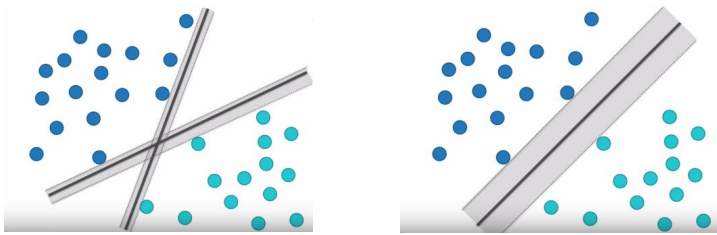
\includegraphics[width=\linewidth]{svms.png}
\end{definition}

\begin{definition}{Hyperplane}\\
In $N$-dimensional space, a hyperplane is a flat affine subspace of dimensions $N-1$. In two dimensions, a hyperplane is a line defined by:
\[b + w_1 x_1 + w_2 x_2 = 0\]
In the general $N$-dimensional case:
\[b + w^T x = 0\]
\end{definition}

\begin{definition}{Support Vectors}\\
    Support vectors are the data points that are closest to the hyperplane and influence its position. They are critical for defining the optimal hyperplane.\\
    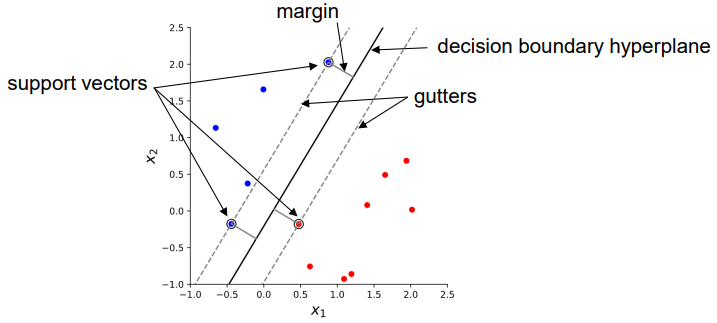
\includegraphics[width=\linewidth]{support_vectors.png}
\end{definition}

\subsection{Mathematical Formulation}

\begin{concept}{Optimisation Task for the Maximal Margin Classifier}\\
    The optimization task for the maximal margin classifier is to minimize the following objective function:
    \[ \min_{\mathbf{w}, b} \frac{1}{2} ||\mathbf{w}||^2 \quad \text{'Primal Form'}\]
    subject to the constraints:
    \[ y^{(m)} (b + \mathbf{w}^T \mathbf{x}^{(m)}) \geq 1, \quad \text{ for } m = 1,..., M \]
    where $\mathbf{w}$ is the weight vector, $b$ is the bias term, and $y^{(m)}$ is the class label of the $m$-th data point.
\end{concept}

\begin{definition}{Maximal Margin Classifier} Primal Form\\
    A maximal margin classifier finds the hyperplane that maximizes the distance to the nearest data point from any class. This leads to the optimization problem:
    \[\min_{b,w} \frac{1}{2}||w||^2\]
    subject to: $y^{(m)}(b + w^T x^{(m)}) \geq 1 \quad \forall m = 1,..., M$

    The data points closest to the hyperplane are called support vectors.
\end{definition}

\begin{concept}{Maximal Margin Classifier} Dual Form\\
The optimization problem for SVMs can be reformulated in its dual form:
\[\max_{\alpha} \mathcal{L}(\alpha) = - \frac{1}{2}\sum_{i=1}^{M}\sum_{j=1}^{M}\alpha_i\alpha_j y^{(i)}y^{(j)}x^{(i)}x^{(j)} + \sum_{m=1}^{M}\alpha_m\]
subject to: $\sum_{m=1}^{M}\alpha_m y^{(m)} = 0$ and $0 \leq \alpha_m \leq C$ for $m = 1, ..., M$

This formulation allows the application of the kernel trick by replacing the dot product $x^{(i)}x^{(j)}$ with a kernel function $\mathcal{K}(x^{(i)}, x^{(j)})$.
\end{concept}

\begin{theorem}{Predictions from the Optimised Lagrangian}\\
    With the optimal $\hat{\alpha}_m$ we can compute the optimal $\widehat{\mathbf{w}}$ from the equation in the previous slide
    \[ \widehat{\mathbf{w}}=\sum_{m=1}^M \hat{\alpha}_m y^{(m)} \mathbf{x}^{(m)} \]
    \[ \text{and }\hat{b}=\frac{1}{M_s} \sum_{m=1}^{M_s}\left(y^{(m)}-\widehat{\mathbf{w}}^T \mathbf{x}^{(m)}\right) \text{ for the support vectors}\]
    where $M_s$ is the number of support vectors and $\quad \hat{\alpha}_m>0$
    \vspace{2mm}\\
    Then, a new sample $\mathbf{x}^{(*)}$ can be classified using $y^{(*)}=\operatorname{sign}(\widehat{\mathbf{w}}^T \mathbf{x}^{(*)}+\hat{b})$
    The distance from the hyperplane can be interpreted as a confidence for the prediction.
\end{theorem}

\subsection{Kernel Trick and Soft Margin}

\begin{concept}{Hard Margin vs. Soft Margin}
\begin{itemize}
    \item \textbf{Hard Margin Classifier}: Requires all points to be correctly classified and outside the margin
    \item \textbf{Soft Margin Classifier}: Allows some points to violate the margin or be misclassified
\end{itemize}
The hard margin classifier works only when data is linearly separable and is sensitive to outliers.
\end{concept}

\begin{definition}{Soft Margin Classifier} Cost Function in Soft-Margin SVM\\
The soft margin classifier allows some data points to violate the margin constraints, adding \textbf{slack variables} $\varepsilon_m \geq 0$:
\[\min_{b,w,\varepsilon} \frac{1}{2}||w||^2 + C\sum_{m=1}^{M}\varepsilon^{(m)}\]
subject to: $y^{(m)}(b + \mathbf{w}^T \mathbf{x}^{(m)}) \geq 1 - \varepsilon^{(m)}$ and $\varepsilon^{(m)} \geq 0$ for $m = 1,..., M$

The parameter $C$ controls the trade-off between maximizing the margin and minimizing constraint violations.\\
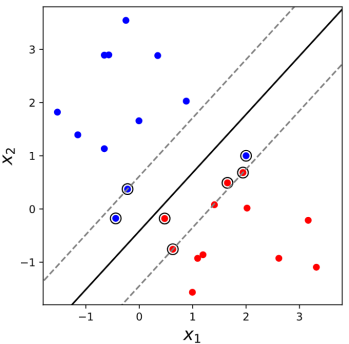
\includegraphics[width=0.5\linewidth]{softmargin_classifier.png}
\end{definition}

\begin{remark}
    Unbalanced data:\\
    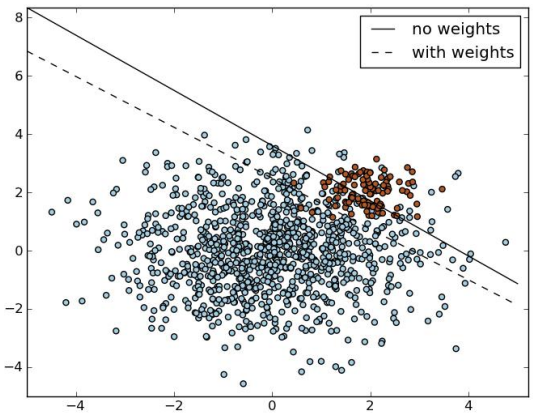
\includegraphics[width=0.5\linewidth]{unbalanced_data.png}
\end{remark}

\begin{example2}{'Wrong' Hyperplane}\\
    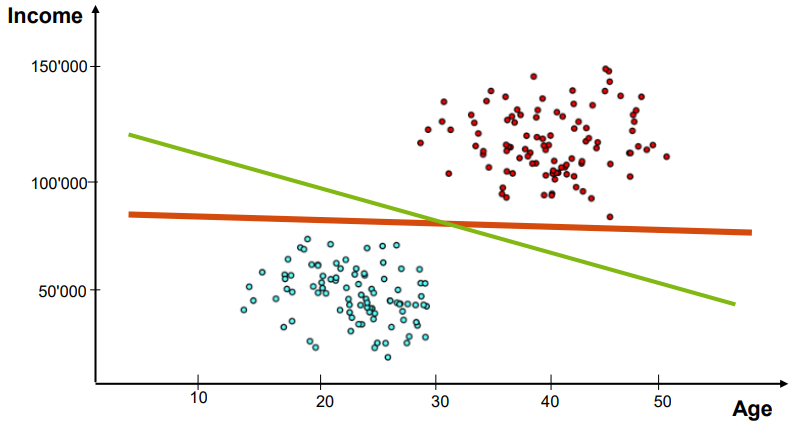
\includegraphics[width=\linewidth]{wrong_hyperplane.png}\\
    The \textcolor{red}{\textbf{RED}} line is the optimal hyperplane for the hard margin classifier. The \textcolor{green}{\textbf{GREEN}} line is NOT optimal!
\end{example2}

\begin{definition}{Standardization and Normalization}\\
    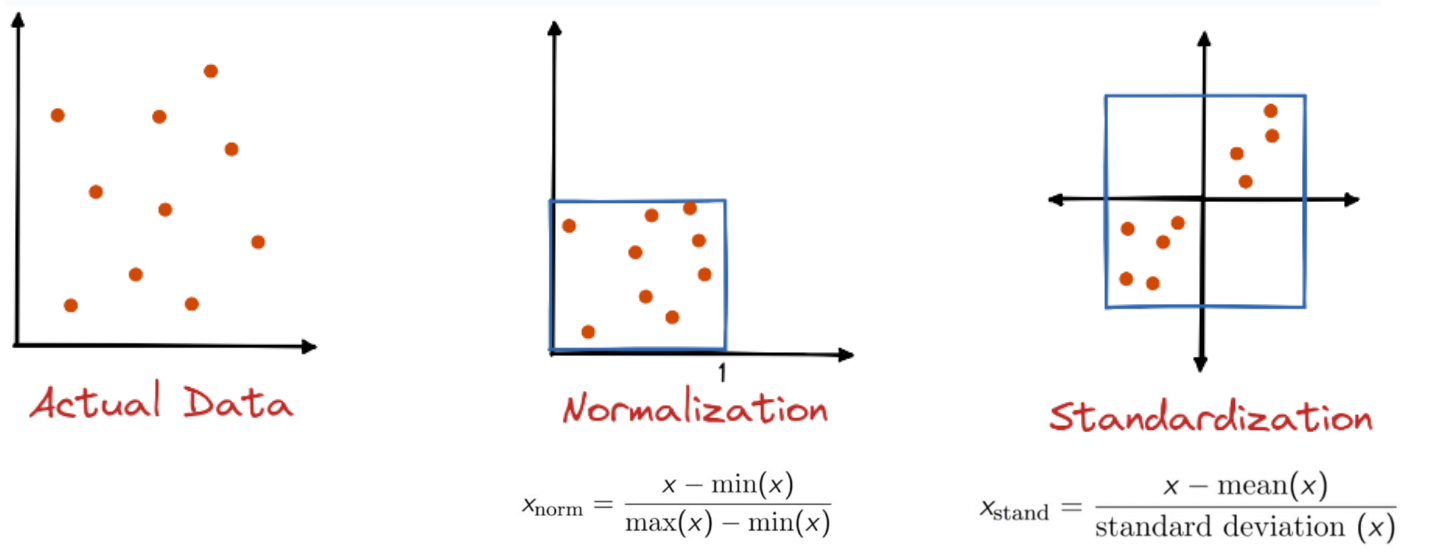
\includegraphics[width=\linewidth]{standardization_normalization.png}\\
    \small Normalization: e.g. for Neural Networks\\
    \small Standardization: e.g. for SVMs, Linear and Logistic Regression    
\end{definition}

\subsubsection{Kernel Trick for non-linearly seperable data}

\begin{definition}{Lifting Trick} Projection to Higher Dimensions\\
    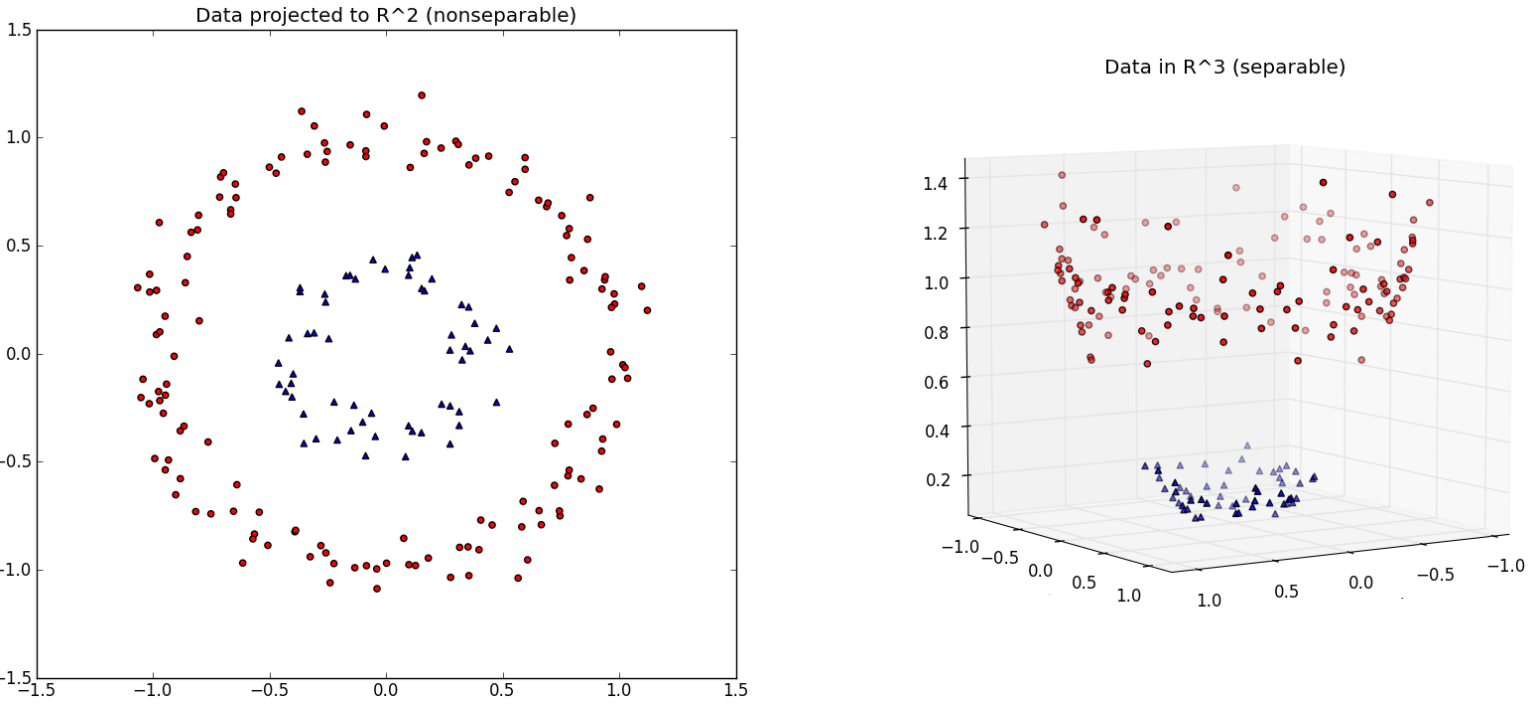
\includegraphics[width=\linewidth]{lifting_trick.png}\\
    Transformation: $(x_1, x_2) \rightarrow (x_1, x_2, x_1^2 + x_2^2)$\\
    \small The lifting trick allows us to transform the data into a higher-dimensional space where it may become linearly separable.
\end{definition}

\begin{concept}{Kernel Trick}\\
The kernel trick allows SVMs to efficiently operate in high-dimensional spaces without explicitly computing the transformation. Common kernels include:
\begin{itemize}
    \item Linear: $\mathcal{K}(x^{(m)}, x^{(m')}) = \sum_{n=1}^{N} x^{(m)}_n x^{(m')}_n$
    \item Polynomial: $\mathcal{K}(x^{(m)}, x^{(m')}) = (1 + \sum_{n=1}^{N} x^{(m)}_n x^{(m')}_n)^d$
    \item RBF: $\mathcal{K}(x^{(m)}, x^{(m')}) = \exp(-\gamma||x^{(m)} - x^{(m')}||^2)$
\end{itemize}
\end{concept}

\begin{theorem}{Maximal Margin Classifier} Dual Form with Kernel Trick
\[\max_{\alpha} \mathcal{L}(\alpha) = - \frac{1}{2}\sum_{i=1}^{M}\sum_{j=1}^{M}\alpha_i\alpha_j y^{(i)}y^{(j)} \textcolor{pink}{\mathcal{K}(x^{(i)}, x^{(j)})} + \sum_{m=1}^{M}\alpha_m\]
subject to: $\sum_{m=1}^{M}\alpha_m y^{(m)} = 0$ and $0 \leq \alpha_m \leq C$ for $m = 1, ..., M$

This formulation allows the application of the kernel trick by replacing the dot product $x^{(i)}x^{(j)}$ with a kernel function $\mathcal{K}(x^{(i)}, x^{(j)})$.
\end{theorem}

\begin{formula}{Common Kernel Functions}

    \begin{minipage}{0.7\linewidth}
    Linear: $\quad K(a, b)=a^{\top} \cdot b$

    Polynomial: $\quad K(a, b)=\left(a^{\top} \cdot b+t\right)^r$ with parameters $\mathbf{t}, \mathbf{r}$

    RBF = Radial Basis Function:
    \[ \mathrm{K}(\mathrm{a}, \mathrm{~b})=e^{-\gamma\|a-b\|^2} \]
    with parameter $\gamma$
    \end{minipage}
    \begin{minipage}{0.25\linewidth}
        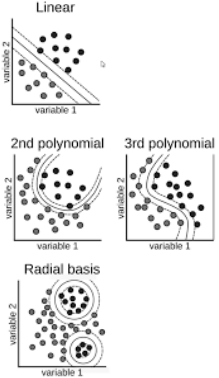
\includegraphics[width=\linewidth]{common_kernel_functions.png}
    \end{minipage}
\end{formula}



\begin{KR}{Selecting the Right Kernel and Parameters}
\paragraph{When to use different kernels}
\begin{itemize}
    \item Linear kernel: 
    \begin{itemize}
        \item When data is linearly separable
        \item When feature space is large compared to sample size
        \item For text classification problems
    \end{itemize}
    \item Polynomial kernel:
    \begin{itemize}
        \item When decision boundary is a curved line or surface
        \item For image processing problems
        \item Typical degrees: 2 or 3
    \end{itemize}
    \item RBF kernel:
    \begin{itemize}
        \item When classes form complex shapes
        \item For most general-purpose classification
        \item When you have sufficient data
    \end{itemize}
\end{itemize}

\paragraph{Parameter tuning}
\begin{itemize}
    \item Use grid search or random search with cross-validation
    \item C parameter search range: $[0.1, 1, 10, 100, 1000]$
    \item For RBF kernel, $\gamma$ search range: $[0.01, 0.1, 1, 10]$
    \item For polynomial kernel, degree values: $[2, 3, 4]$
\end{itemize}

\paragraph{Optimize for the metric that matters}
\begin{itemize}
    \item Accuracy for balanced problems
    \item F1-score for imbalanced problems
    \item Precision or recall when false positives or false negatives are more critical
\end{itemize}
\end{KR}

\begin{definition}{RBF Kernel}
    \[ \mathrm{K}(\mathrm{a}, \mathrm{~b}) = e^{-\gamma\|a-b\|^2} = e^{-\frac{||a-b||^2}{2\sigma^2}} \]
    Small $\gamma \rightarrow$ large width $\sigma$ (Gaussian kernel)\\
    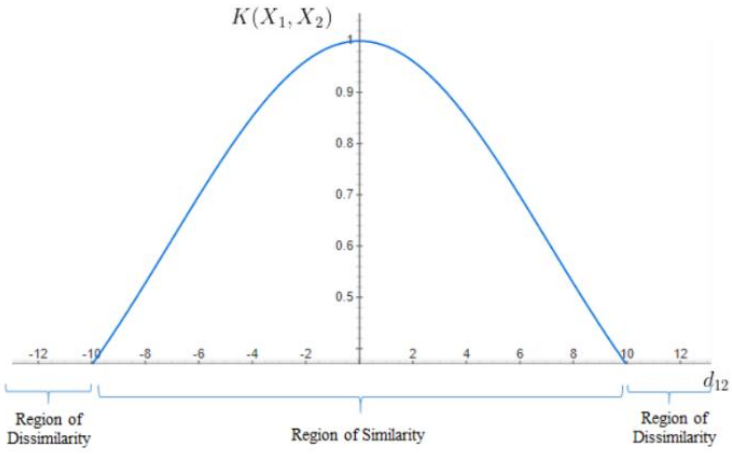
\includegraphics[width=\linewidth]{small_gamma.png}\\
    Large $\gamma \rightarrow$ small width $\sigma$ (Gaussian kernel)\\
    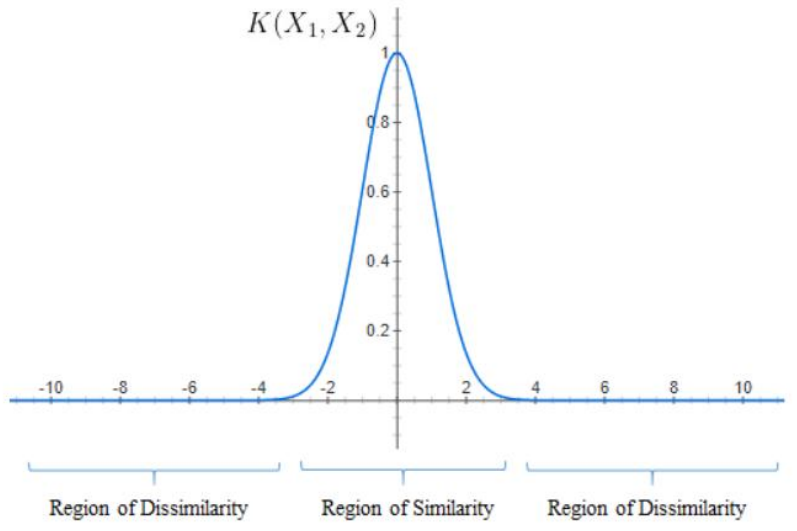
\includegraphics[width=\linewidth]{large_gamma.png}
\end{definition}

\begin{example2}{RBF Kernel}\\
    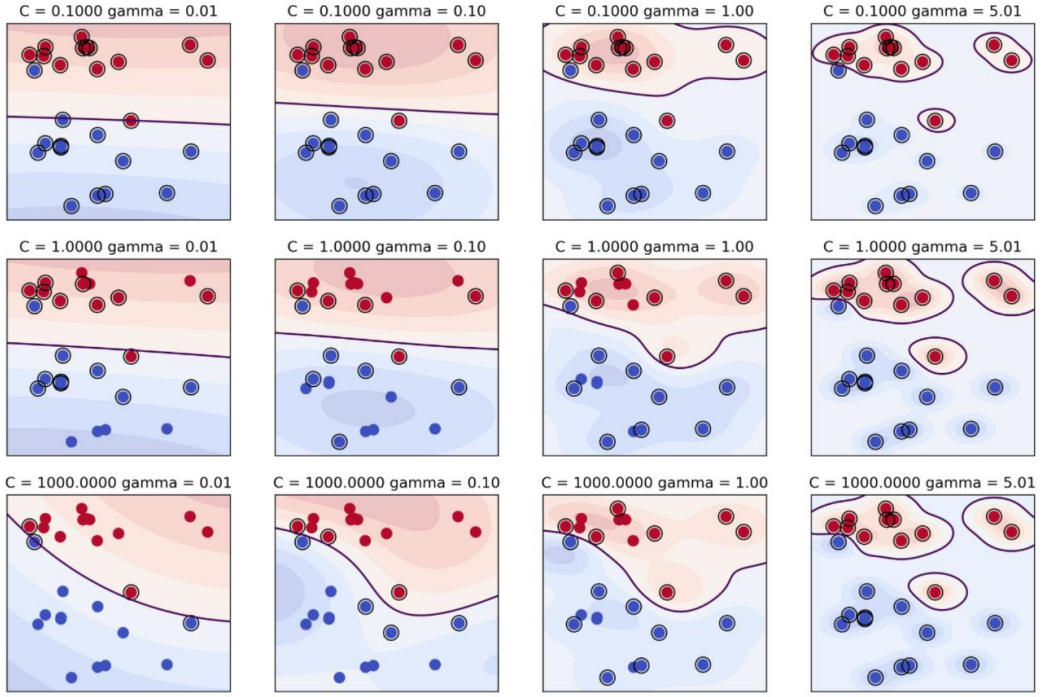
\includegraphics[width=\linewidth]{rbfkernel.png}
\end{example2}

\begin{theorem}{Interdependence of SVM Hyperparameters}\\
    $C$ and $\gamma$ both influence the shape of the decision boundary and need to be tuned together 
    using hyperparameter optimization (e.g. via cross validation)
\end{theorem}

\begin{example2}{ConceptTest: RBF Kernel}\\
    In the SVM below we are using $\mathrm{C}=1$. Which image has the highest value for hyperparameter $\gamma$ ?

    \[ K\left(\mathbf{x}, \mathbf{x}^{(m)}\right)=\exp \left(-\gamma\left\|\mathbf{x}^{(m)}-\mathbf{x}\right\|^2\right) \]

    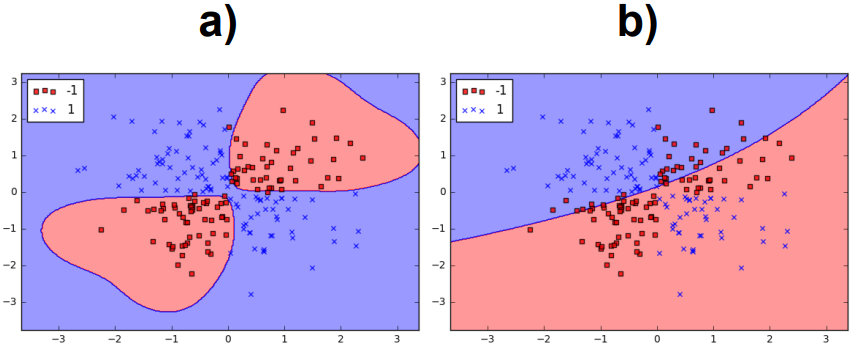
\includegraphics[width=\linewidth]{rbfexample1.png}\\
    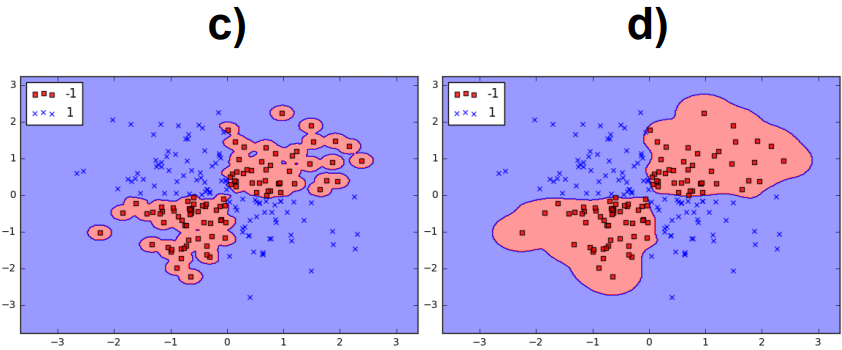
\includegraphics[width=\linewidth]{rbfexample2.png}
\end{example2}

\begin{example}{SVM Application} Linear Kernel\\
Consider classifying flowers based on petal length and width:
\begin{itemize}
    \item Features: Petal length ($x_1$) and petal width ($x_2$)
    \item Classes: Setosa (-1) and Versicolor (+1)
    \item After training with a linear kernel, we get $b = -0.5$ and $w = [0.2, 0.8]$
    \item For a new flower with petal length = 4 cm and width = 1.3 cm:
    \begin{itemize}
        \item $f(x) = -0.5 + 0.2 \times 4 + 0.8 \times 1.3 = -0.5 + 0.8 + 1.04 = 1.34 > 0$
        \item Prediction: Versicolor (class +1)
    \end{itemize}
\end{itemize}
\end{example}

\begin{KR}{Training a Support Vector Machine}
    \paragraph{Select kernel}
    Choose an appropriate kernel function:
    \begin{itemize}
        \item Linear kernel for linearly separable data
        \item Polynomial kernel for more complex, non-linear boundaries
        \item RBF (Gaussian) kernel for highly non-linear data
    \end{itemize}
    
    \paragraph{Select hyperparameters}
    \begin{itemize}
        \item $C$: Regularization parameter (controls trade-off between margin width and misclassification)
        \item Kernel parameters: degree $d$ for polynomial kernel, $\gamma$ for RBF kernel
    \end{itemize}
    
    \paragraph{Train the model}
    \begin{itemize}
        \item Set up the optimization problem to maximize the margin
        \item Solve the quadratic programming problem to find support vectors
    \end{itemize}
    
    \paragraph{Make predictions}
    For a new data point $x$:
    \begin{itemize}
        \item Compute $f(x) = b + \sum_{i \in SV} \alpha_i y_i K(x_i, x)$
        \item Predict class 1 if $f(x) > 0$, otherwise class -1
    \end{itemize}
    \end{KR}

\subsection{Multi-class Classification with SVMs}

\begin{concept}{Multi-class SVM}\\
SVMs are inherently binary classifiers. For multi-class problems, approaches include:
\begin{itemize}
    \item \textbf{One-vs-All}: Train $K$ SVMs, each separating one class from all others
    \item \textbf{One-vs-One}: Train $\binom{K}{2}$ SVMs, each separating one class from another
\end{itemize}
\end{concept}

\begin{definition}{One-vs-All (One-vs-Rest) Approach}\\
In the one-vs-all approach:
\begin{itemize}
    \item Train $K$ binary classifiers, one for each class
    \item For each classifier, positive examples are from one class, negative examples from all other classes
    \item For prediction, apply all classifiers and select the class with highest confidence (furthest from the decision boundary)
\end{itemize}
\end{definition}

\begin{definition}{One-vs-One Approach}\\
In the one-vs-one approach:
\begin{itemize}
    \item Train $\binom{K}{2} = \frac{K(K-1)}{2}$ binary classifiers, one for each pair of classes
    \item For prediction, each classifier votes for one class
    \item The class with the most votes wins
\end{itemize}
\end{definition}

\begin{example2}{Multi-class Classification}\\
Consider a flower classification problem with three classes: Setosa, Versicolor, and Virginica.
\begin{itemize}
    \item Features: Petal length and petal width
    \item One-vs-All approach:
    \begin{itemize}
        \item Classifier 1: Setosa vs. non-Setosa
        \item Classifier 2: Versicolor vs. non-Versicolor
        \item Classifier 3: Virginica vs. non-Virginica
    \end{itemize}
    \item One-vs-One approach:
    \begin{itemize}
        \item Classifier 1: Setosa vs. Versicolor
        \item Classifier 2: Setosa vs. Virginica
        \item Classifier 3: Versicolor vs. Virginica
    \end{itemize}
\end{itemize}
\tcblower
For a new flower with petal length = 5 cm and width = 1.8 cm:

One-vs-All approach:
\begin{itemize}
    \item Classifier 1 (Setosa vs. rest): $f_1(x) = -3.5 < 0$ (not Setosa)
    \item Classifier 2 (Versicolor vs. rest): $f_2(x) = -0.8 < 0$ (not Versicolor)
    \item Classifier 3 (Virginica vs. rest): $f_3(x) = 2.3 > 0$ (Virginica)
\end{itemize}
Prediction: Virginica

One-vs-One approach:
\begin{itemize}
    \item Classifier 1 (Setosa vs. Versicolor): Votes for Versicolor
    \item Classifier 2 (Setosa vs. Virginica): Votes for Virginica
    \item Classifier 3 (Versicolor vs. Virginica): Votes for Virginica
\end{itemize}
Virginica gets 2 votes, Versicolor gets 1 vote, Setosa gets 0 votes.
Prediction: Virginica
\end{example2}

\subsection{SVM for Regression}

\begin{definition}{Support Vector Regression (SVR)}\\
SVR applies the same principles as SVM to regression tasks by:
\begin{itemize}
    \item Fitting as many instances as possible on a "street" with width controlled by parameter $\varepsilon$
    \item Allowing some points to be off the street (margin violations)
    \item Using kernels to handle non-linear regression tasks
\end{itemize}
\end{definition}

\begin{concept}{Key Differences Between SVR and Linear Regression}
\begin{itemize}
    \item Linear regression minimizes the squared error for all points
    \item SVR is only concerned with errors larger than $\varepsilon$ (the tube width)
    \item SVR is more robust to outliers
    \item SVR produces a sparse solution (depends only on support vectors)
\end{itemize}
\end{concept}

\begin{KR}{Implementing Support Vector Regression}
\paragraph{Define the problem}
\begin{itemize}
    \item Determine if a non-linear relationship exists in the data
    \item Decide if robustness to outliers is important
\end{itemize}

\paragraph{Select parameters}
\begin{itemize}
    \item $\varepsilon$: Controls the width of the insensitive tube (larger $\varepsilon$ means fewer support vectors)
    \item $C$: Regularization parameter (smaller $C$ means more regularization)
    \item Kernel and its parameters (same as for SVM classification)
\end{itemize}

\paragraph{Train and evaluate}
\begin{itemize}
    \item Train using appropriate solver
    \item Evaluate using metrics like MSE, MAE, or $R^2$
    \item Tune parameters using cross-validation
\end{itemize}
\end{KR}

\begin{example}{SVR Example}
Consider predicting house prices based on size (in square feet):
\begin{itemize}
    \item Training data: 100 houses with sizes ranging from 1000 to 3000 sq ft and prices from \$200,000 to \$600,000
    \item We use SVR with an RBF kernel, $C=1000$, $\varepsilon=10000$, and $\gamma=0.0001$
    \item For a new house with 2500 sq ft:
    \begin{itemize}
        \item Predicted price: \$475,000
        \item Only 15 support vectors were used for this prediction (out of 100 training examples)
    \end{itemize}
\end{itemize}
\end{example}


% NOTE: Add SVM margin visualization showing support vectors and decision boundary

\begin{concept}{SVM Classifier Family}
\begin{itemize}
    \item \textbf{Maximal margin hyperplane classifier}: for linearly separable data
    \item \textbf{Support vector classifier}: for almost linearly separable data (soft margin)
    \item \textbf{Support vector machine}: for non-linearly separable data (with kernel trick)
\end{itemize}
\end{concept}

\begin{KR}{SVM Implementation Process}\\
\paragraph{Step 1: Data analysis}
Start with data in a relatively low dimension and assess linear separability

\paragraph{Step 2: Kernel selection}
If data is not linearly separable, transform data into a higher dimension using kernels

\paragraph{Step 3: Optimization}
Find a Support Vector Classifier that separates the transformed data with maximum margin

\paragraph{Step 4: Hyperparameter tuning}
Optimize C parameter and kernel parameters using cross-validation
\end{KR}

% NOTE: Add 3D transformation visualization showing 2D non-separable data becoming 3D separable

\subsection{Hyperparameter Effects}

\begin{concept}{C Parameter Effects}\\
The C parameter controls the trade-off between margin maximization and classification errors:
\begin{itemize}
    \item \textbf{Small C}: Wide margin, more misclassifications allowed (high bias, low variance)
    \item \textbf{Large C}: Narrow margin, fewer misclassifications allowed (low bias, high variance)
\end{itemize}
\end{concept}

% NOTE: Add four panels showing different C values and their effects on margin and misclassification
	\raggedcolumns
	\pagebreak
	\section{Decision Trees and Random Forests}

\subsection{Predictions from Decision Trees}

\begin{definition}{Decision Tree}\\
A decision tree is a tree-like model of decisions where:
\begin{itemize}
    \item Each internal node represents a test on a feature
    \item Each branch represents an outcome of the test
    \item Each leaf node represents a prediction (class label or value)
\end{itemize}
Decision trees can be used for both classification and regression tasks.
\end{definition}

\begin{definition}{Gini Impurity}\\
Gini impurity measures how often a randomly chosen element would be incorrectly labeled if labeled randomly according to the distribution of labels in the subset:
\[G(Q_i) = 1 - \sum_{k=1}^{K} p_{i,k}^2\]
where $p_{i,k}$ is the proportion of class $k$ observations in node $i$.
\end{definition}

\begin{definition}{Entropy}\\
Entropy is another measure of impurity:
\[H(Q_i) = -\sum_{k=1}^{K} p_{i,k} \log_2 p_{i,k}\]
Both Gini impurity and entropy are used in building decision trees.
\end{definition}

\begin{concept}{Node Purity and Splitting Criteria}\\
When building a decision tree, nodes are split to maximize "purity":
\begin{itemize}
    \item A pure node contains only samples of a single class
    \item Splits are chosen to maximize information gain
    \item Information gain is the reduction in impurity (Gini or entropy) after a split
    \item The cost of a split is the weighted average of child node impurities:
    \[J(Q_i, \theta) = \frac{m^{left}_i}{m_i}G(Q^{left}_i(\theta)) + \frac{m^{right}_i}{m_i}G(Q^{right}_i(\theta))\]
\end{itemize}
\end{concept}

\begin{KR}{Making Predictions with Decision Trees}\\
\paragraph{For classification}
Follow the tree from root to leaf:
\begin{itemize}
    \item Start at the root node
    \item At each internal node, evaluate the feature test
    \item Follow the branch corresponding to the test outcome
    \item Continue until reaching a leaf node
    \item Return the majority class in the leaf as the prediction
\end{itemize}

\paragraph{For regression}
Follow the same process, but:
\begin{itemize}
    \item Return the average target value of training samples in the leaf
    \item Trees approximate the target function as a piecewise constant function
\end{itemize}

\paragraph{Prediction confidence}
For classification:
\begin{itemize}
    \item Confidence can be estimated from class proportions in the leaf
    \item For example, if a leaf has 80 samples of class A and 20 of class B:
    \begin{itemize}
        \item Predict class A with 80\% confidence
        \item Alternative: predict probabilities [0.8, 0.2]
    \end{itemize}
\end{itemize}
\end{KR}

\begin{example}{Decision Tree Classification}
Consider classifying iris flowers based on petal length and width:
\begin{itemize}
    \item Root node: "Is petal length < 2.45 cm?"
    \item If yes: Predict Setosa (all samples with petal length < 2.45 cm are Setosa)
    \item If no: "Is petal width < 1.75 cm?"
    \item If yes: Predict Versicolor
    \item If no: Predict Virginica
\end{itemize}
\end{example}

\subsection{Training Decision Trees}

\begin{KR}{Training a Decision Tree with CART Algorithm}\\
\paragraph{Start with root node}
Begin with all training samples in the root node

\paragraph{Find best split}
For each feature and potential threshold:
\begin{itemize}
    \item Calculate the cost function (e.g., Gini impurity or entropy for classification, MSE for regression)
    \item Choose the feature and threshold that minimizes the cost
\end{itemize}

\paragraph{Split the node}
Divide the data based on the best split found

\paragraph{Recursively build sub-trees}
For each child node, repeat steps 2-3 until stopping criteria are met:
\begin{itemize}
    \item Maximum depth reached
    \item Minimum samples per node threshold met
    \item Node becomes pure (all samples belong to same class)
\end{itemize}

\paragraph{Make predictions}
For classification: Predict the majority class in the leaf node
For regression: Predict the average value of samples in the leaf node
\end{KR}

\begin{concept}{Building Binary Trees}\\
The CART algorithm builds binary trees:
\begin{itemize}
    \item Each split creates exactly two child nodes (binary split)
    \item For categorical features with $p$ possible values, there are $2^{p-1} - 1$ possible binary partitions
    \item In practice, often use one-hot encoding for categorical features
\end{itemize}
\end{concept}

\begin{example2}{Training a Decision Tree}\\
Consider a dataset with two features (age and income) and a binary target (buy vs. don't buy):
\begin{itemize}
    \item 10 samples: 6 "buy" and 4 "don't buy"
    \item Root node Gini impurity: $1 - (\frac{6}{10})^2 - (\frac{4}{10})^2 = 1 - 0.36 - 0.16 = 0.48$
\end{itemize}
\tcblower
Evaluate split on age = 30:
\begin{itemize}
    \item Left node (age < 30): 5 samples, 4 "buy" and 1 "don't buy"
    \item Left node Gini: $1 - (\frac{4}{5})^2 - (\frac{1}{5})^2 = 1 - 0.64 - 0.04 = 0.32$
    \item Right node (age $\leq$ 30): 5 samples, 2 "buy" and 3 "don't buy"
    \item Right node Gini: $1 - (\frac{2}{5})^2 - (\frac{3}{5})^2 = 1 - 0.16 - 0.36 = 0.48$
    \item Weighted Gini after split: $\frac{5}{10} \times 0.32 + \frac{5}{10} \times 0.48 = 0.16 + 0.24 = 0.40$
    \item Information gain: $0.48 - 0.40 = 0.08$
\end{itemize}

Evaluate split on income = 50K:
\begin{itemize}
    \item Left node (income < 50K): 6 samples, 2 "buy" and 4 "don't buy"
    \item Left node Gini: $1 - (\frac{2}{6})^2 - (\frac{4}{6})^2 = 1 - 0.11 - 0.44 = 0.45$
    \item Right node (income $leq$ 50K): 4 samples, 4 "buy" and 0 "don't buy"
    \item Right node Gini: $1 - (\frac{4}{4})^2 - (\frac{0}{4})^2 = 1 - 1 - 0 = 0$
    \item Weighted Gini after split: $\frac{6}{10} \times 0.45 + \frac{4}{10} \times 0 = 0.27 + 0 = 0.27$
    \item Information gain: $0.48 - 0.27 = 0.21$
\end{itemize}

The split on income = 50K has higher information gain, so it's selected for the root node.
\end{example2}

\subsection{Regularization in Decision Trees}

\begin{concept}{Regularization in Decision Trees}\\
Decision trees tend to overfit without regularization. Common regularization techniques include:
\begin{itemize}
    \item \textbf{Max depth}: Limit the maximum depth of the tree
    \item \textbf{Min samples split}: Require minimum number of samples to split a node
    \item \textbf{Min samples leaf}: Require minimum number of samples in leaf nodes
    \item \textbf{Max features}: Limit number of features considered for splitting
    \item \textbf{Pruning}: Remove branches that don't improve generalization
\end{itemize}
\end{concept}

\begin{KR}{Pruning Decision Trees}\\
\paragraph{Pre-pruning (early stopping)}
Stop growing the tree early by setting constraints:
\begin{itemize}
    \item Maximum depth
    \item Minimum samples required for splitting
    \item Minimum samples required in leaf nodes
    \item Minimum impurity decrease required for splitting
\end{itemize}

\paragraph{Post-pruning}
Grow a full tree, then prune back branches:
\begin{itemize}
    \item Grow a full, deep tree
    \item Evaluate performance on validation set
    \item Iteratively remove branches that don't improve validation performance
    \item Continue until pruning no longer improves performance
\end{itemize}

\paragraph{Cost-complexity pruning}
A systematic approach to post-pruning:
\begin{itemize}
    \item Define a cost-complexity measure that balances tree complexity and error
    \item Generate a sequence of trees with decreasing complexity
    \item Select the tree with best validation performance
\end{itemize}
\end{KR}

\begin{concept}{White Box vs. Black Box Models}\\
Decision trees are considered "white box" models because:
\begin{itemize}
    \item The decision-making process is transparent and interpretable
    \item You can see the exact rules and thresholds used for classification
    \item Each prediction can be explained by tracing the path through the tree
\end{itemize}
This contrasts with "black box" models like neural networks, where the decision-making process is opaque.
\end{concept}

\subsection{Random Forests}

\begin{definition}{Random Forest}\\
Random Forest is an ensemble learning method that combines multiple decision trees to improve prediction accuracy and control overfitting. Key aspects include:
\begin{itemize}
    \item Each tree is trained on a bootstrap sample of the training data (random sampling with replacement)
    \item When building trees, only a random subset of features is considered for splitting at each node
    \item Final prediction is made by averaging predictions (regression) or taking majority vote (classification) from all trees
\end{itemize}
\end{definition}

\begin{concept}{Bagging (Bootstrap Aggregating)}\\
Bagging is a technique to improve model stability and accuracy:
\begin{itemize}
    \item Generate multiple training sets by sampling with replacement from the original training data
    \item Train a separate model on each bootstrap sample
    \item Combine predictions by averaging (regression) or voting (classification)
    \item Reduces variance without increasing bias
\end{itemize}
\end{concept}

\begin{concept}{Out-of-Bag Evaluation}\\
In Random Forests, each tree is trained on a bootstrap sample, leaving some samples out (out-of-bag or OOB samples):
\begin{itemize}
    \item OOB samples act as a validation set for each tree
    \item For each sample, predictions are made only by trees that didn't use it for training
    \item OOB error provides an unbiased estimate of the generalization error
\end{itemize}
\end{concept}

\begin{KR}{Training a Random Forest}\\
\paragraph{Initialize the forest}
\begin{itemize}
    \item Define number of trees $n\_trees$
    \item Set parameters: max\_features, max\_depth, min\_samples\_leaf, etc.
\end{itemize}

\paragraph{Build individual trees}
For each tree:
\begin{itemize}
    \item Create bootstrap sample from training data
    \item Build decision tree considering only random subset of features at each split
\end{itemize}

\paragraph{Make predictions}
For a new data point:
\begin{itemize}
    \item Get prediction from each tree
    \item Aggregate predictions (average for regression, majority vote for classification)
\end{itemize}
\end{KR}

\begin{concept}{Feature Importance in Random Forests}\\
Random forests provide a natural way to measure feature importance:
\begin{itemize}
    \item For each feature, measure the increase in prediction error after permuting its values
    \item Features with large increases in error are more important
    \item Alternatively, measure the average decrease in impurity across all trees when a feature is used for splitting
\end{itemize}
This helps identify which features have the most predictive power.
\end{concept}

\begin{example}{Random Forest Application}
Consider a credit scoring application:
\begin{itemize}
    \item Task: Predict if a customer will default on a loan
    \item Features: Income, age, employment history, credit history, loan amount
    \item Model: Random forest with 100 trees
    \item Each tree uses a bootstrap sample (about 63\% of training data)
    \item At each node, only $\sqrt{5} \approx 2$ features are considered for splitting
    \item Results:
    \begin{itemize}
        \item Individual tree accuracy: 78-85\%
        \item Random forest accuracy: 92\%
        \item Feature importance: Credit history (40\%), income (25\%), loan amount (20\%), employment history (10\%), age (5\%)
    \end{itemize}
\end{itemize}
\end{example}

\begin{KR}{Tuning Random Forest Hyperparameters}\\
\paragraph{Number of trees (n\_estimators)}
\begin{itemize}
    \item Start with a large number (100-500)
    \item More trees generally improves performance but increases computation
    \item Performance often plateaus after a certain number
\end{itemize}

\paragraph{Maximum features (max\_features)}
\begin{itemize}
    \item For classification: Default is $\sqrt{n\_features}$
    \item For regression: Default is $n\_features/3$
    \item Try different values and use cross-validation
\end{itemize}

\paragraph{Tree constraints}
\begin{itemize}
    \item max\_depth: Controls maximum depth of trees
    \item min\_samples\_split: Minimum samples required to split
    \item min\_samples\_leaf: Minimum samples required in leaf nodes
\end{itemize}

\paragraph{Bootstrap options}
\begin{itemize}
    \item bootstrap: Whether to use bootstrap samples (True by default)
    \item max\_samples: Size of bootstrap samples
\end{itemize}
\end{KR}

\begin{concept}{Other Tree-Based Ensemble Methods}\\
Beyond random forests, other tree-based ensemble methods include:
\begin{itemize}
    \item \textbf{Extra Trees (Extremely Randomized Trees)}: Similar to random forests but uses random thresholds for splitting
    \item \textbf{Gradient Boosting}: Builds trees sequentially, each correcting errors of previous trees
    \item \textbf{AdaBoost (Adaptive Boosting)}: Focuses subsequent trees on examples previous trees misclassified
    \item \textbf{XGBoost, LightGBM, CatBoost}: Optimized implementations of gradient boosting
\end{itemize}
\end{concept}
	\raggedcolumns
	\pagebreak
	\section{Generative Models and Naive Bayes}
	\raggedcolumns
	\pagebreak
	\section{Clustering}
	\raggedcolumns
	\pagebreak
	\section{Neural Networks}

Neural networks are a powerful class of models inspired by the human brain, capable of learning complex patterns from data. This section covers their structure, training methods, and advanced applications.

\subsection{Feed-Forward Neural Networks}

Feed-forward neural networks are the foundation of deep learning, consisting of layers of interconnected neurons that process information in one direction.

\begin{definition}{Neural Network}\\
A neural network is a computational model inspired by the human brain. The basic building block is the neuron, which computes a weighted sum of its inputs, adds a bias term, and applies an activation function:
\[a = \zeta(w^T x + b)\]
where:
\begin{itemize}
    \item $a$ is the neuron's output (activation)
    \item $x$ is the input vector
    \item $w$ is the weight vector
    \item $b$ is the bias
    \item $\zeta$ is the activation function
\end{itemize}
\end{definition}

\begin{definition}{Feed-forward Neural Network}\\
Feed-forward neural networks consist of neurons organized in layers:
\begin{itemize}
    \item Input layer: Passes input features to the network
    \item Hidden layers: Process information through weighted connections
    \item Output layer: Produces the final prediction
\end{itemize}
Information flows in one direction, from input to output, with no cycles/loops.
\end{definition}

\begin{definition}{Softmax Regression}\\
Softmax regression generalizes logistic regression to multi-class classification:
\begin{itemize}
    \item For each class, it computes a separate linear combination of the inputs
    \item It applies the softmax function to get probabilities for each class: $softmax(z)_k = \frac{\exp(z_k)}{\sum_{i=1}^{K} \exp(z_i)}$
    \item The predicted class is the one with the highest probability
\end{itemize}
\end{definition}

\begin{definition}{Activation Functions}\\
Common activation functions include:
\begin{itemize}
    \item Sigmoid: $\zeta(z) = \frac{1}{1 + e^{-z}}$, outputs in range (0,1)
    \item Tanh: $\zeta(z) = \frac{e^z - e^{-z}}{e^z + e^{-z}}$, outputs in range (-1,1)
    \item ReLU: $\zeta(z) = \max(0, z)$, simple and computationally efficient
    \item Softmax: $\zeta(z_i) = \frac{e^{z_i}}{\sum_{j} e^{z_j}}$, used for multi-class classification
\end{itemize}
\end{definition}

\begin{concept}{Universality Theorem}\\
The universality theorem (Hornik, 1991) states that a neural network with a single hidden layer using a nonlinear activation function can approximate any continuous function to any desired level of accuracy, given enough hidden units.

This means neural networks are very flexible and can learn complex relationships in data, though deeper networks with multiple hidden layers often learn more efficiently.
\end{concept}

\subsection{Training Neural Networks}

Training neural networks involves finding optimal weights and biases that minimize the difference between predicted and actual outputs.

\begin{definition}{Cost Functions for Neural Networks}\\
Common cost functions include:
\begin{itemize}
    \item For regression: Mean Squared Error (MSE)
    \item For binary classification: Binary Cross-Entropy
    \item For multi-class classification: Categorical Cross-Entropy
\end{itemize}
\end{definition}

\begin{definition}{Backpropagation}\\
Backpropagation is the algorithm used to train neural networks by:
\begin{enumerate}
    \item Performing a forward pass to compute predictions
    \item Computing the error/loss
    \item Propagating the error backwards through the network to compute gradients
    \item Updating weights and biases using gradient descent
\end{enumerate}
This process leverages the chain rule of calculus to efficiently compute gradients.
\end{definition}

\begin{KR}{Training a Neural Network}\\
\paragraph{Initialize the network}
\begin{itemize}
    \item Define network architecture (number of layers, neurons per layer)
    \item Initialize weights and biases randomly
    \item Select activation functions, cost function, and optimizer
\end{itemize}

\paragraph{Forward propagation}
For each training sample:
\begin{itemize}
    \item Input features to the first layer
    \item Compute activations through each layer
    \item Obtain prediction from output layer
\end{itemize}

\paragraph{Compute loss}
Calculate the difference between predictions and actual values using the cost function

\paragraph{Backpropagation}
\begin{itemize}
    \item Compute gradients of the cost function with respect to weights and biases
    \item Use chain rule to propagate gradients backward through the network
\end{itemize}

\paragraph{Update weights}
\begin{itemize}
    \item Use gradient descent or an advanced optimizer (Adam, RMSprop)
    \item Update weights and biases: $w = w - \alpha \frac{\partial L}{\partial w}$
\end{itemize}

\paragraph{Repeat}
Iterate steps 2-5 until convergence or for a fixed number of epochs
\end{KR}

\begin{example2}{Backpropagation Example}\\
Consider a simple neural network with one input, one hidden layer with two neurons, and one output neuron.
\begin{itemize}
    \item Input: $x = 0.5$
    \item Hidden layer weights: $w^{(1)}_{11} = 0.15, w^{(1)}_{21} = 0.25$
    \item Hidden layer biases: $b^{(1)}_1 = 0.35, b^{(1)}_2 = 0.45$
    \item Output layer weights: $w^{(2)}_{11} = 0.40, w^{(2)}_{12} = 0.50$
    \item Output layer bias: $b^{(2)}_1 = 0.60$
    \item Activation function: Sigmoid
    \item True output: $y = 0.75$
\end{itemize}
\tcblower
Forward pass:
\begin{align*}
z^{(1)}_1 &= w^{(1)}_{11} \cdot x + b^{(1)}_1 = 0.15 \cdot 0.5 + 0.35 = 0.425\\
a^{(1)}_1 &= \sigma(z^{(1)}_1) = \sigma(0.425) = 0.605\\
z^{(1)}_2 &= w^{(1)}_{21} \cdot x + b^{(1)}_2 = 0.25 \cdot 0.5 + 0.45 = 0.575\\
a^{(1)}_2 &= \sigma(z^{(1)}_2) = \sigma(0.575) = 0.640\\
z^{(2)}_1 &= w^{(2)}_{11} \cdot a^{(1)}_1 + w^{(2)}_{12} \cdot a^{(1)}_2 + b^{(2)}_1\\
&= 0.40 \cdot 0.605 + 0.50 \cdot 0.640 + 0.60 = 0.842 + 0.60 = 1.442\\
\hat{y} = a^{(2)}_1 &= \sigma(z^{(2)}_1) = \sigma(1.442) = 0.809
\end{align*}

Backpropagation:
\begin{align*}
\frac{\partial L}{\partial a^{(2)}_1} &= 2(a^{(2)}_1 - y) = 2(0.809 - 0.75) = 0.118\\
\frac{\partial a^{(2)}_1}{\partial z^{(2)}_1} &= a^{(2)}_1(1 - a^{(2)}_1) = 0.809 \cdot 0.191 = 0.154\\
\frac{\partial L}{\partial z^{(2)}_1} &= \frac{\partial L}{\partial a^{(2)}_1} \cdot \frac{\partial a^{(2)}_1}{\partial z^{(2)}_1} = 0.118 \cdot 0.154 = 0.018
\end{align*}

This gradient is then used to update the weights in the network.
\end{example2}

\subsection{Neural Network Architectures}

Neural networks come in various architectures, each designed for specific types of data or tasks.

\begin{definition}{Common Neural Network Architectures}\\
\begin{itemize}
    \item \textbf{Fully Connected (Dense) Network}: Each neuron is connected to all neurons in adjacent layers
    \item \textbf{Convolutional Neural Network (CNN)}: Uses convolutional layers to process grid-like data (e.g., images)
    \item \textbf{Recurrent Neural Network (RNN)}: Contains loops to persist information, suitable for sequential data
    \item \textbf{Long Short-Term Memory (LSTM)}: A special type of RNN that can learn long-term dependencies
    \item \textbf{Transformer}: Uses attention mechanisms, effective for sequential data like text
\end{itemize}
\end{definition}

\begin{concept}{Convolutional Neural Networks}\\
CNNs are specialized for processing grid-like data such as images:
\begin{itemize}
    \item \textbf{Convolutional layers}: Apply filters to detect local patterns
    \item \textbf{Pooling layers}: Reduce spatial dimensions while retaining important features
    \item \textbf{Parameter sharing}: Same filter applied across the entire input
    \item \textbf{Local connectivity}: Each neuron connects to a small region of the input
\end{itemize}
These properties make CNNs highly effective for tasks like image classification, object detection, and image segmentation.
\end{concept}

\begin{concept}{Recurrent Neural Networks}\\
RNNs are designed for sequential data:
\begin{itemize}
    \item Each neuron receives input from the current sample and its own previous output
    \item This creates a form of memory that captures dependencies across time steps
    \item Useful for tasks like time series prediction, speech recognition, and language modeling
    \item Variants like LSTM and GRU address the vanishing gradient problem in standard RNNs
\end{itemize}
\end{concept}

\subsection{Preventing Overfitting}

Overfitting occurs when a model learns the training data too well, including its noise, and fails to generalize to new data. Several techniques can prevent this issue in neural networks.

\begin{concept}{Dealing with Overfitting in Neural Networks}\\
Techniques to prevent overfitting include:
\begin{itemize}
    \item \textbf{Dropout}: Randomly deactivate neurons during training
    \item \textbf{Early Stopping}: Stop training when performance on validation set starts to degrade
    \item \textbf{Data Augmentation}: Create new training samples by applying transformations
    \item \textbf{Regularization}: Add penalty terms for large weights
\end{itemize}
\end{concept}

\begin{definition}{Dropout}\\
Dropout is a regularization technique that prevents overfitting in neural networks:
\begin{itemize}
    \item During training, randomly deactivate a fraction of neurons in each layer
    \item Each forward and backward pass uses a different randomly dropped network
    \item Forces the network to learn redundant representations
    \item During inference, all neurons are used (with scaled activations)
\end{itemize}
\end{definition}

\begin{definition}{Early Stopping}\\
Early stopping prevents overfitting by monitoring performance on a validation set:
\begin{itemize}
    \item Train the model and evaluate on validation set periodically
    \item Stop training when validation error starts to increase
    \item Use the model parameters from the point with best validation performance
\end{itemize}
\end{definition}

\begin{definition}{Data Augmentation}\\
Data augmentation increases the effective size of the training dataset:
\begin{itemize}
    \item For images: rotations, flips, crops, color adjustments
    \item For text: synonym replacement, back-translation
    \item For audio: time stretching, pitch shifting, masking
\end{itemize}
\end{definition}

\begin{KR}{Implementing Dropout}\\
\paragraph{During training}
\begin{itemize}
    \item For each training batch, generate a binary mask for each layer with dropout
    \item Set a dropout rate (typically 0.2-0.5) representing the fraction of neurons to drop
    \item Multiply activations by the mask to zero out dropped neurons
    \item Scale remaining activations by $\frac{1}{1-\text{dropout\_rate}}$ to maintain same expected value
\end{itemize}

\paragraph{During testing/inference}
\begin{itemize}
    \item Use all neurons without dropout
    \item No scaling needed if scaling was done during training
\end{itemize}

\paragraph{Implementation considerations}
\begin{itemize}
    \item Apply dropout after activation functions
    \item Use different dropout rates for different layers (typically higher for layers with more neurons)
    \item Don't apply dropout to the output layer
\end{itemize}
\end{KR}

\begin{concept}{Vanishing and Exploding Gradient Problems}\\
In deep networks, gradients can become very small (vanishing) or very large (exploding) as they propagate through the network:
\begin{itemize}
    \item \textbf{Vanishing gradients}: Parameters in early layers change very slowly or not at all
    \item \textbf{Exploding gradients}: Parameters in early layers change dramatically, causing instability
    \item \textbf{Causes}: Repeated multiplication of values less than 1 (vanishing) or greater than 1 (exploding)
\end{itemize}
Solutions include:
\begin{itemize}
    \item Better activation functions (ReLU, Leaky ReLU)
    \item Weight initialization techniques (Xavier, He initialization)
    \item Batch normalization
    \item Residual connections (skip connections)
\end{itemize}
\end{concept}

\subsection{Hyperparameter Tuning}

Hyperparameters are settings that control the training process and model architecture. Choosing optimal values is crucial for model performance.

\begin{KR}{Choosing Hyperparameters for Neural Networks}\\
\paragraph{Architecture design}
\begin{itemize}
    \item Number of layers: Start small and increase gradually
    \item Neurons per layer: Powers of 2 (64, 128, 256) work well; larger for complex tasks
    \item Activation functions: ReLU for hidden layers, softmax for multi-class output
\end{itemize}

\paragraph{Training parameters}
\begin{itemize}
    \item Learning rate: Start with 0.01 or 0.001 and tune using learning rate finder
    \item Batch size: 32, 64, or 128 for most tasks; larger if memory allows
    \item Optimizer: Adam is a good default choice
    \item Epochs: Use early stopping with patience
\end{itemize}

\paragraph{Regularization}
\begin{itemize}
    \item Dropout rate: 0.2-0.5 depending on layer size
    \item Weight decay (L2 regularization): 1e-4 is a reasonable starting point
    \item Early stopping patience: 10-20 epochs
\end{itemize}

\paragraph{Advanced techniques}
\begin{itemize}
    \item Learning rate schedules: Reduce on plateau or cosine annealing
    \item Batch normalization: Apply before activation functions
    \item Skip connections: Use for networks deeper than 10 layers
\end{itemize}
\end{KR}

\begin{concept}{Cross-Validation for Neural Networks}\\
Cross-validation helps find optimal hyperparameters:
\begin{itemize}
    \item Split data into training, validation, and test sets
    \item Train models with different hyperparameter combinations
    \item Evaluate each model on validation set
    \item Select hyperparameters that yield best validation performance
    \item Final evaluation on test set
\end{itemize}
Unlike traditional k-fold cross-validation, neural networks often use a single validation split due to computational constraints.
\end{concept}

\begin{example}{Digit Recognition with Neural Networks}
Consider the MNIST dataset of handwritten digits:
\begin{itemize}
    \item Input: 28x28 pixel grayscale images (784 features)
    \item Output: 10 classes (digits 0-9)
    \item Network architecture:
    \begin{itemize}
        \item Input layer: 784 neurons
        \item Hidden layer 1: 128 neurons with ReLU activation
        \item Hidden layer 2: 64 neurons with ReLU activation
        \item Output layer: 10 neurons with softmax activation
    \end{itemize}
    \item Training:
    \begin{itemize}
        \item Loss function: Categorical cross-entropy
        \item Optimizer: Adam with learning rate 0.001
        \item Batch size: 64
        \item Epochs: 20 with early stopping
    \end{itemize}
    \item Results:
    \begin{itemize}
        \item Training accuracy: 99.2\%
        \item Validation accuracy: 98.1\%
    \end{itemize}
\end{itemize}
\end{example}

\subsection{Advanced Topics}

Neural networks continue to evolve with advanced techniques that improve performance, efficiency, and applicability to various domains.

\begin{concept}{Transfer Learning}\\
Transfer learning leverages knowledge from pre-trained models:
\begin{itemize}
    \item Start with a model trained on a large dataset
    \item Remove the final layer(s) and replace with new layers
    \item Either freeze pre-trained layers or fine-tune them with a small learning rate
    \item Requires much less data than training from scratch
    \item Common in computer vision (ResNet, VGG) and NLP (BERT, GPT)
\end{itemize}
\end{concept}

\begin{definition}{Batch Normalization}\\
Batch normalization normalizes the inputs of each layer:
\begin{itemize}
    \item Normalizes activations to have mean 0 and variance 1
    \item Reduces internal covariate shift
    \item Allows higher learning rates
    \item Acts as a regularizer
    \item Applied before or after activation functions
\end{itemize}
\end{definition}

\begin{concept}{Advanced Optimizers}\\
Beyond standard gradient descent, advanced optimizers improve training:
\begin{itemize}
    \item \textbf{Momentum}: Adds a fraction of previous update to current update
    \item \textbf{RMSprop}: Adapts learning rates based on recent gradients
    \item \textbf{Adam}: Combines momentum and RMSprop
    \item \textbf{AdamW}: Adam with decoupled weight decay
\end{itemize}
\end{concept}

\begin{KR}{Implementing Transfer Learning}\\
\paragraph{Select pre-trained model}
\begin{itemize}
    \item Choose model trained on a relevant domain
    \item Consider model size, accuracy, and compatibility
    \item Common options: ResNet, VGG, EfficientNet for images; BERT, GPT for text
\end{itemize}

\paragraph{Prepare the model}
\begin{itemize}
    \item Load pre-trained weights
    \item Remove the output layer (and possibly some layers before it)
    \item Add new layers specific to your task
\end{itemize}

\paragraph{Training approach}
\begin{itemize}
    \item Feature extraction: Freeze pre-trained layers, train only new layers
    \item Fine-tuning: Train the entire network with a small learning rate
    \item Progressive fine-tuning: Gradually unfreeze more layers
\end{itemize}

\paragraph{Adapt to your data}
\begin{itemize}
    \item Ensure input preprocessing matches pre-trained model
    \item Consider domain adaptation techniques if domains differ significantly
    \item Use appropriate regularization for new layers
\end{itemize}
\end{KR}

\begin{example2}{Practical Neural Network Project}\\
Consider an image classification task to identify plant diseases from leaf images:
\begin{itemize}
    \item Dataset: 5,000 images across 10 disease categories
    \item Limited computational resources
\end{itemize}
\tcblower
Solution approach using transfer learning:
\begin{itemize}
    \item Base model: Pre-trained ResNet50 (trained on ImageNet)
    \item Remove top classification layer
    \item Add custom layers:
    \begin{itemize}
        \item Global average pooling
        \item Dropout layer (rate=0.3)
        \item Dense layer with 256 neurons and ReLU activation
        \item Final layer with 10 neurons and softmax activation
    \end{itemize}
    \item Training strategy:
    \begin{itemize}
        \item First stage: Freeze ResNet layers, train only custom layers (5 epochs)
        \item Second stage: Unfreeze last 30 ResNet layers, train entire model with small learning rate (0.0001) for 15 epochs
    \end{itemize}
    \item Data augmentation:
    \begin{itemize}
        \item Random rotations (±20°)
        \item Horizontal and vertical flips
        \item Small zoom and brightness variations
    \end{itemize}
    \item Results: 96.5\% accuracy on test set, compared to 85\% when training from scratch
\end{itemize}
\end{example2}

\begin{concept}{Model Interpretability}\\
Techniques to understand neural network decisions:
\begin{itemize}
    \item \textbf{Feature importance}: Quantifying the impact of each input feature
    \item \textbf{Activation visualization}: Examining neuron activations for different inputs
    \item \textbf{Saliency maps}: Highlighting regions of input that most influence the output
    \item \textbf{LIME (Local Interpretable Model-agnostic Explanations)}: Approximating the model locally with an interpretable model
    \item \textbf{SHAP (SHapley Additive exPlanations)}: Assigning each feature an importance value
\end{itemize}
Interpretability helps build trust, debug models, and identify potential biases.
\end{concept}

\begin{KR}{Debugging Neural Networks}\\
\paragraph{Diagnose learning problems}
\begin{itemize}
    \item Monitor training and validation losses
    \item If validation loss increases while training loss decreases: Overfitting
    \item If both losses plateau at high values: Underfitting
    \item If both losses are unstable: Learning rate may be too high
\end{itemize}

\paragraph{Check gradients}
\begin{itemize}
    \item Inspect gradient magnitudes; very large or very small values indicate problems
    \item Test with gradient clipping to prevent exploding gradients
    \item Verify with numerical gradient checking in critical cases
\end{itemize}

\paragraph{Analyze model predictions}
\begin{itemize}
    \item Examine confusion matrix to identify patterns in misclassifications
    \item Look at the most confidently wrong predictions
    \item Test with simpler inputs to verify basic functionality
\end{itemize}

\paragraph{Simplify and rebuild}
\begin{itemize}
    \item Start with a minimal working model
    \item Add complexity incrementally
    \item Establish baseline performance with simple models
    \item Verify each component individually
\end{itemize}
\end{KR}
	\raggedcolumns
\end{multicols}
\end{document}